\section{路段}

\begin{frame}{情人節要做什麼}
\begin{center}
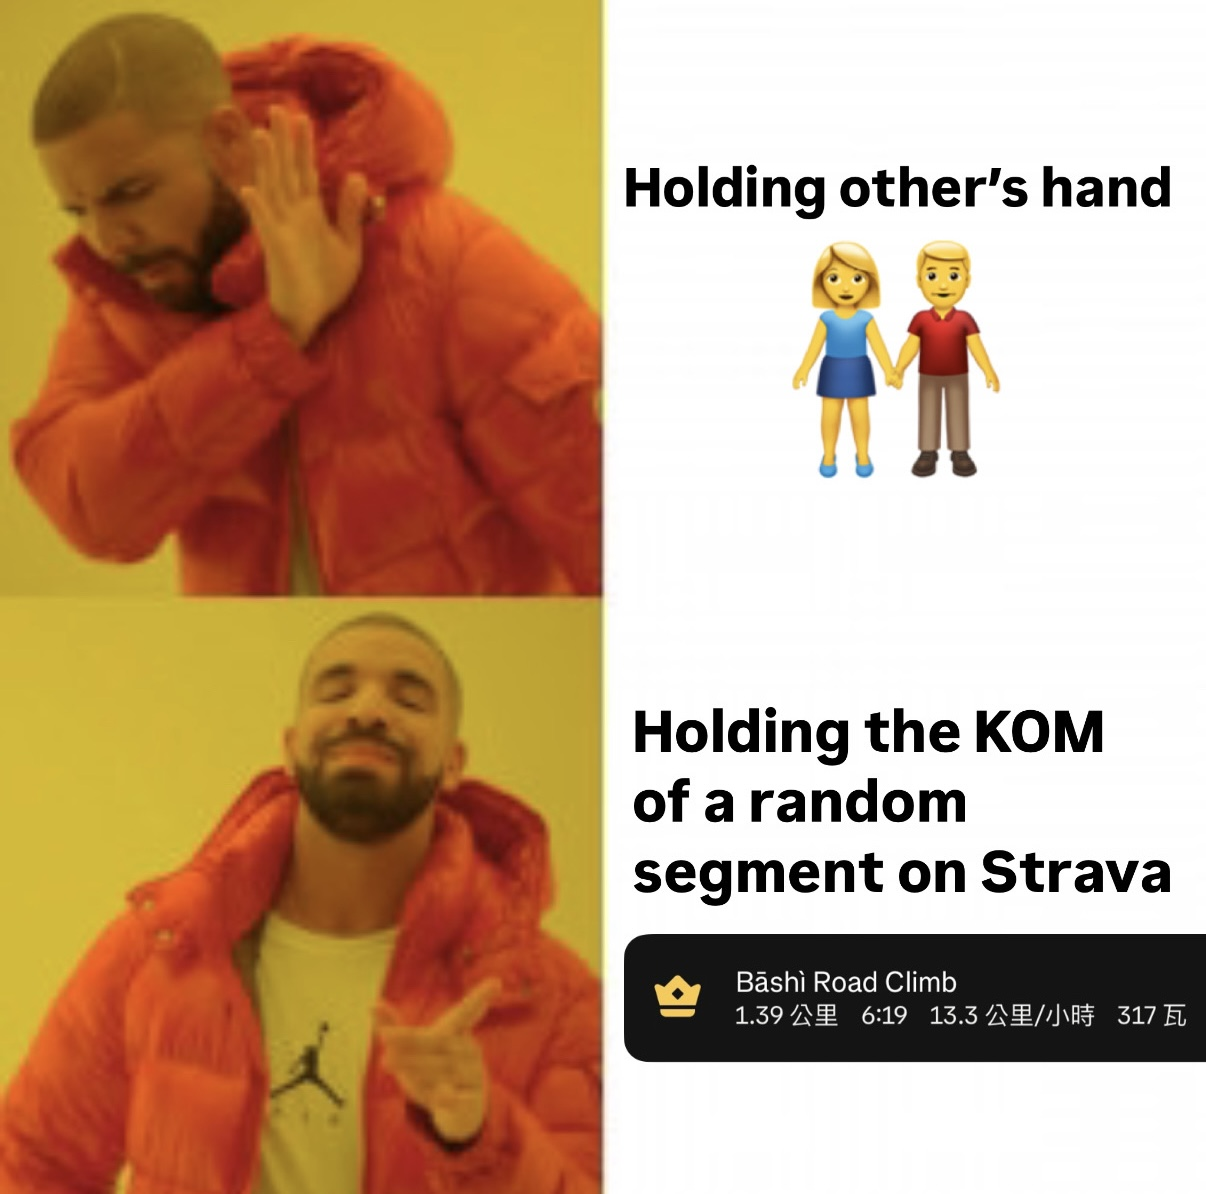
\includegraphics[height=7cm]{holdmeme.JPG}
\end{center}
\end{frame}

\begin{frame}{路段 (Segment)}
\begin{itemize}
\item 一條大家常常騎的路
\item 通常是爬坡、比賽路線
\item 可以比較大家的成績
\item 常見路段:\href{https://brianhsu7476.github.io/segmentsExplorer/}{Segments Explorer}
\item 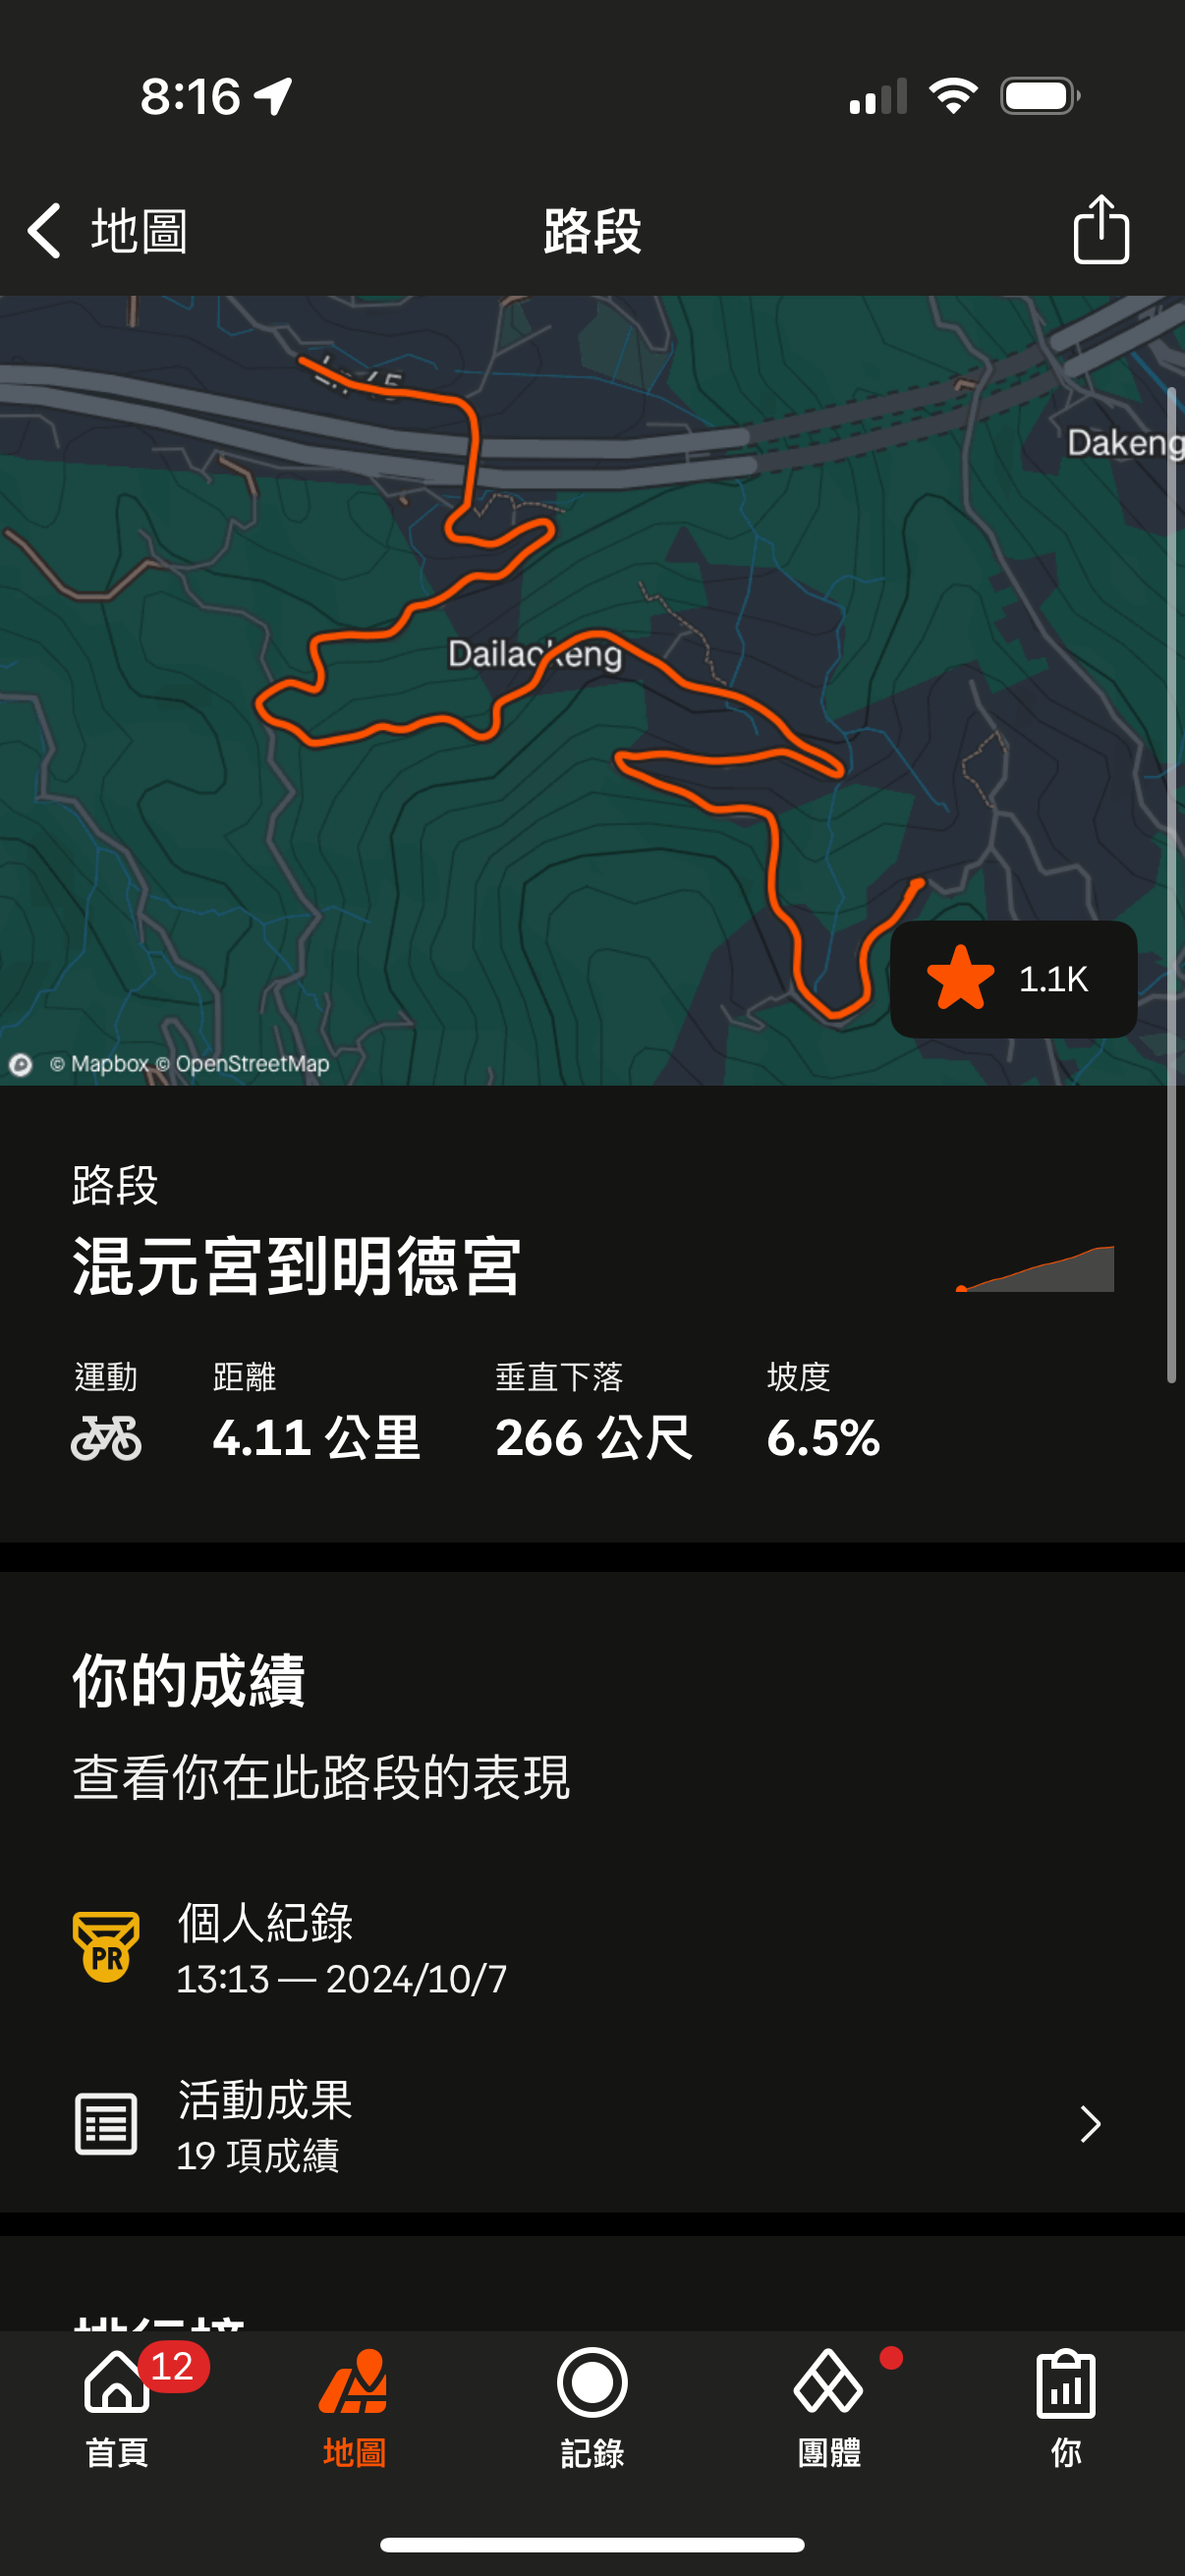
\includegraphics[height=5cm]{maokongSegment.png}
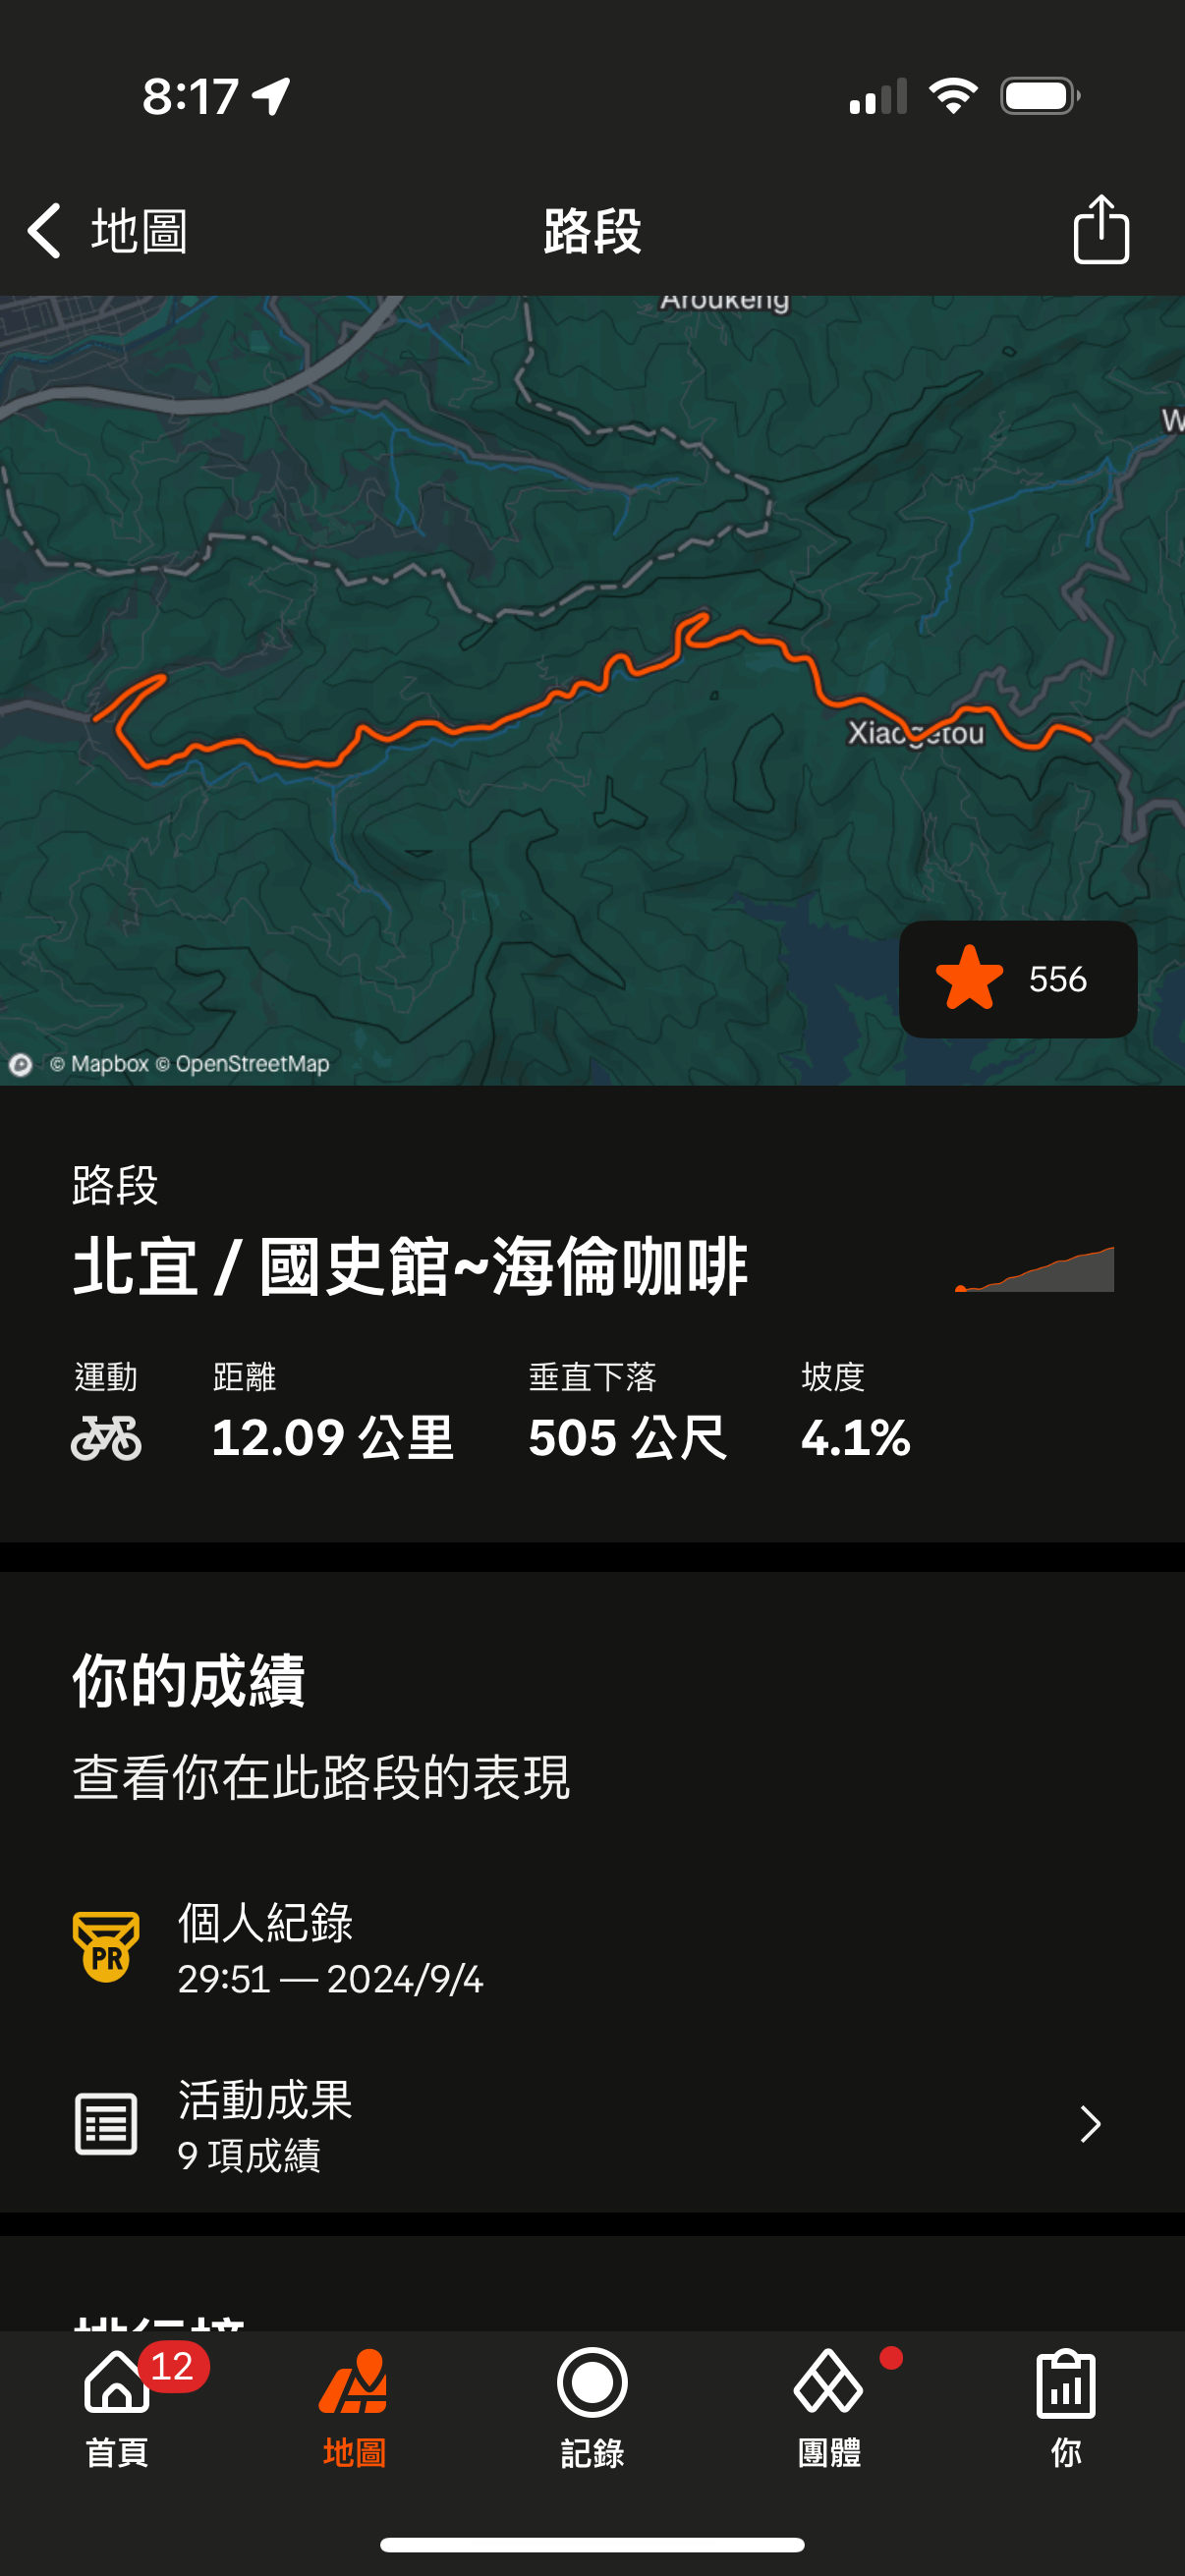
\includegraphics[height=5cm]{coffeeSegment.png}
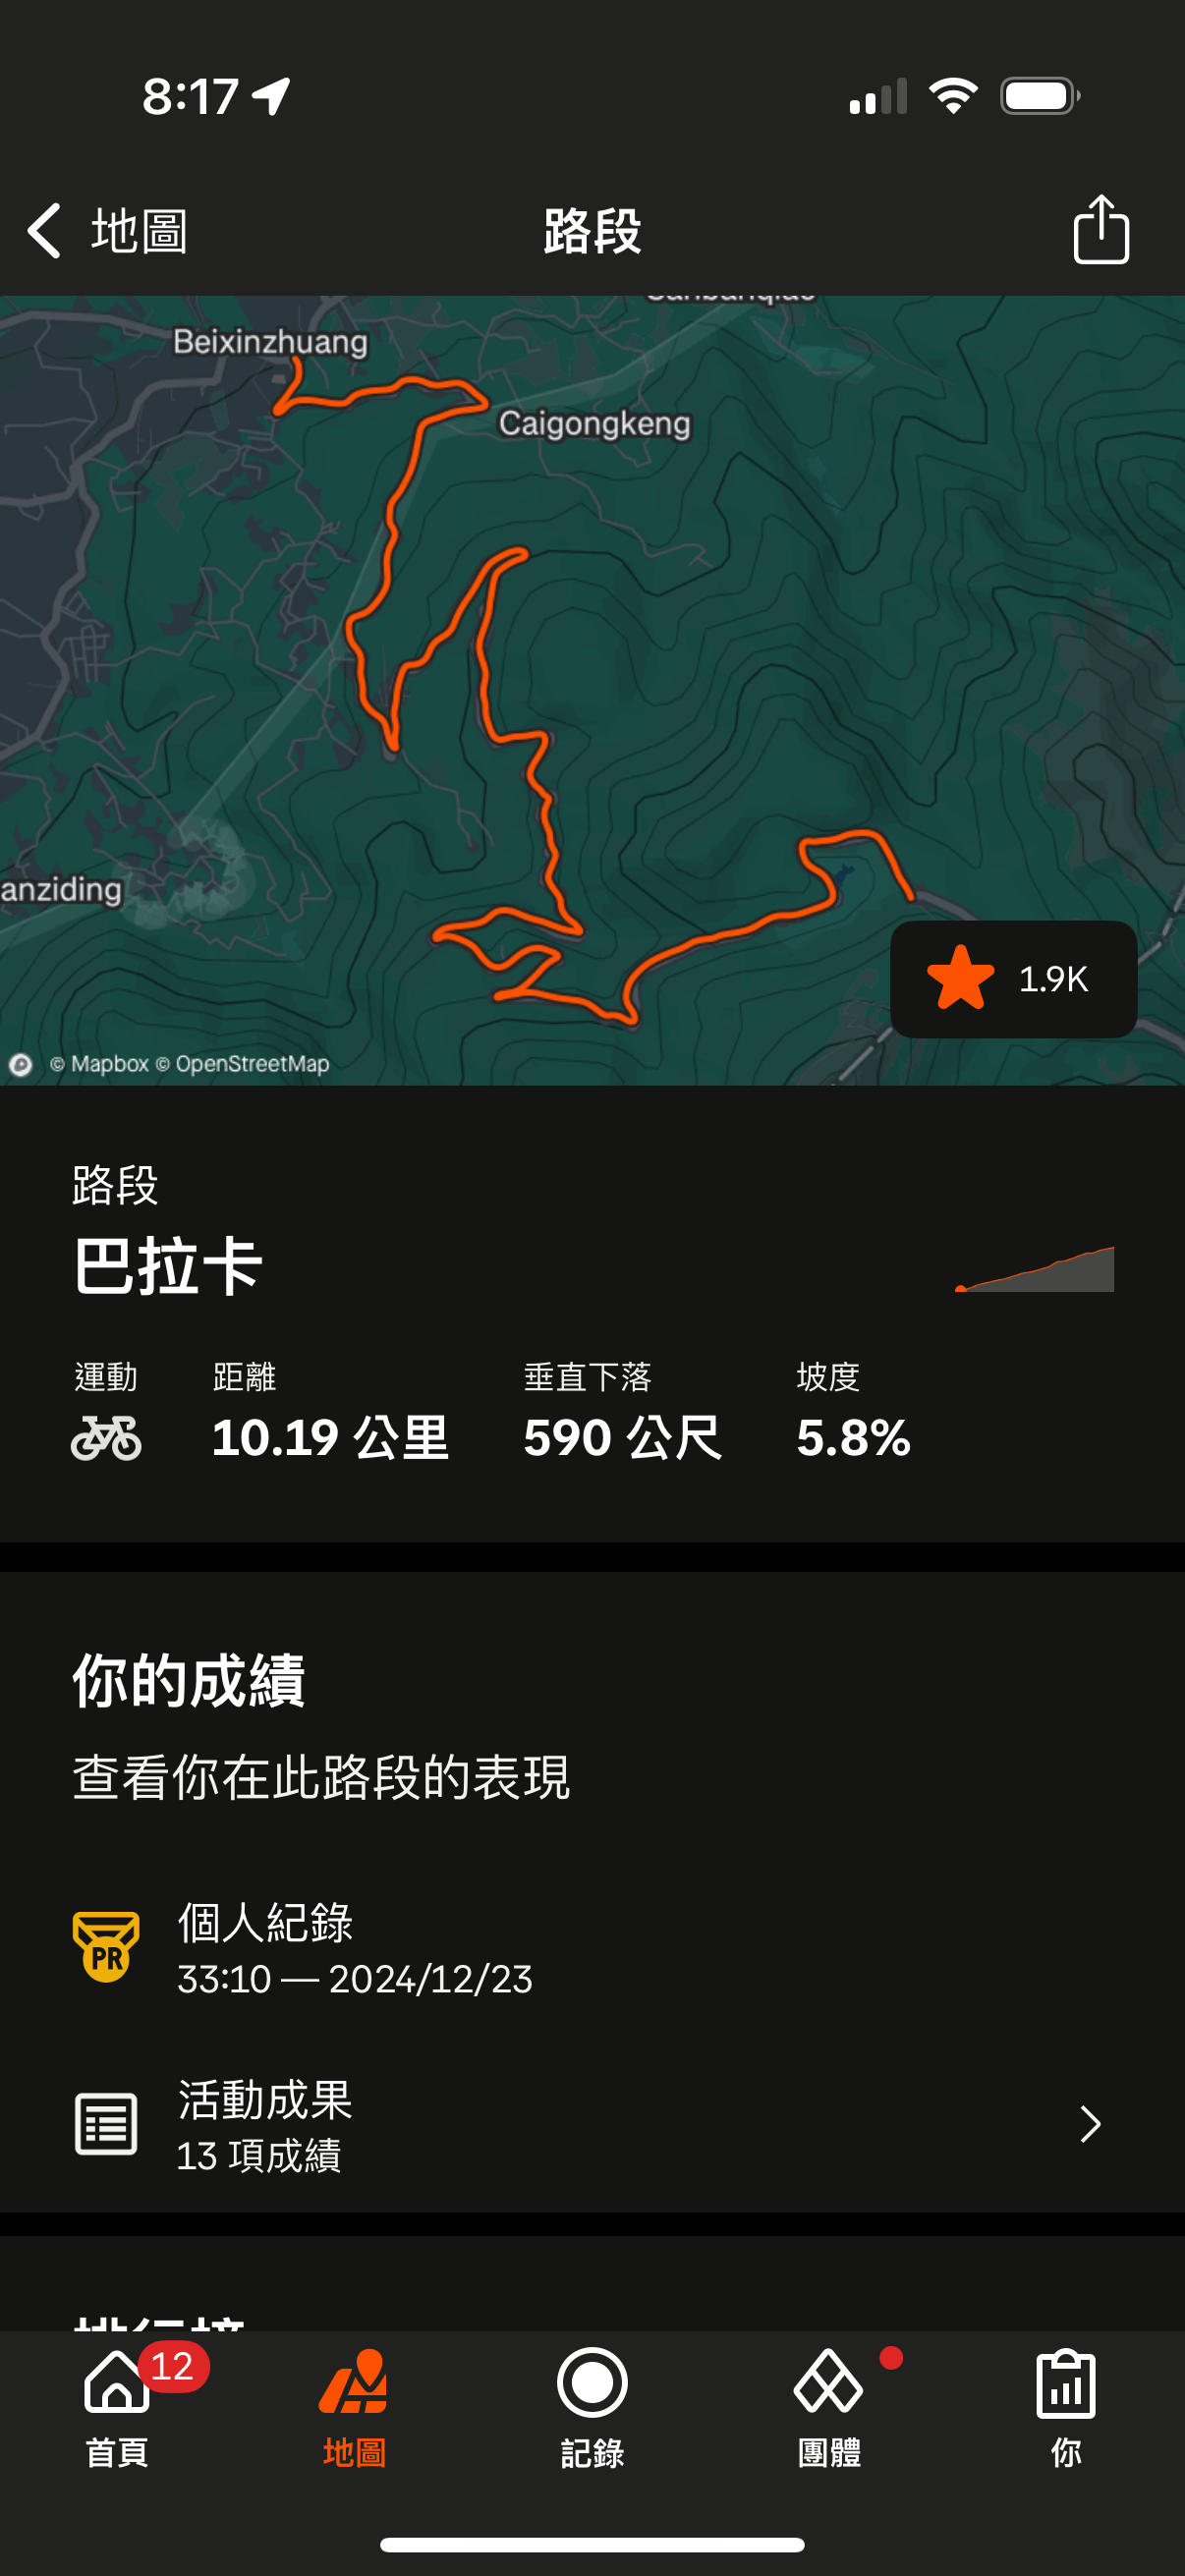
\includegraphics[height=5cm]{balakaSegment.png}
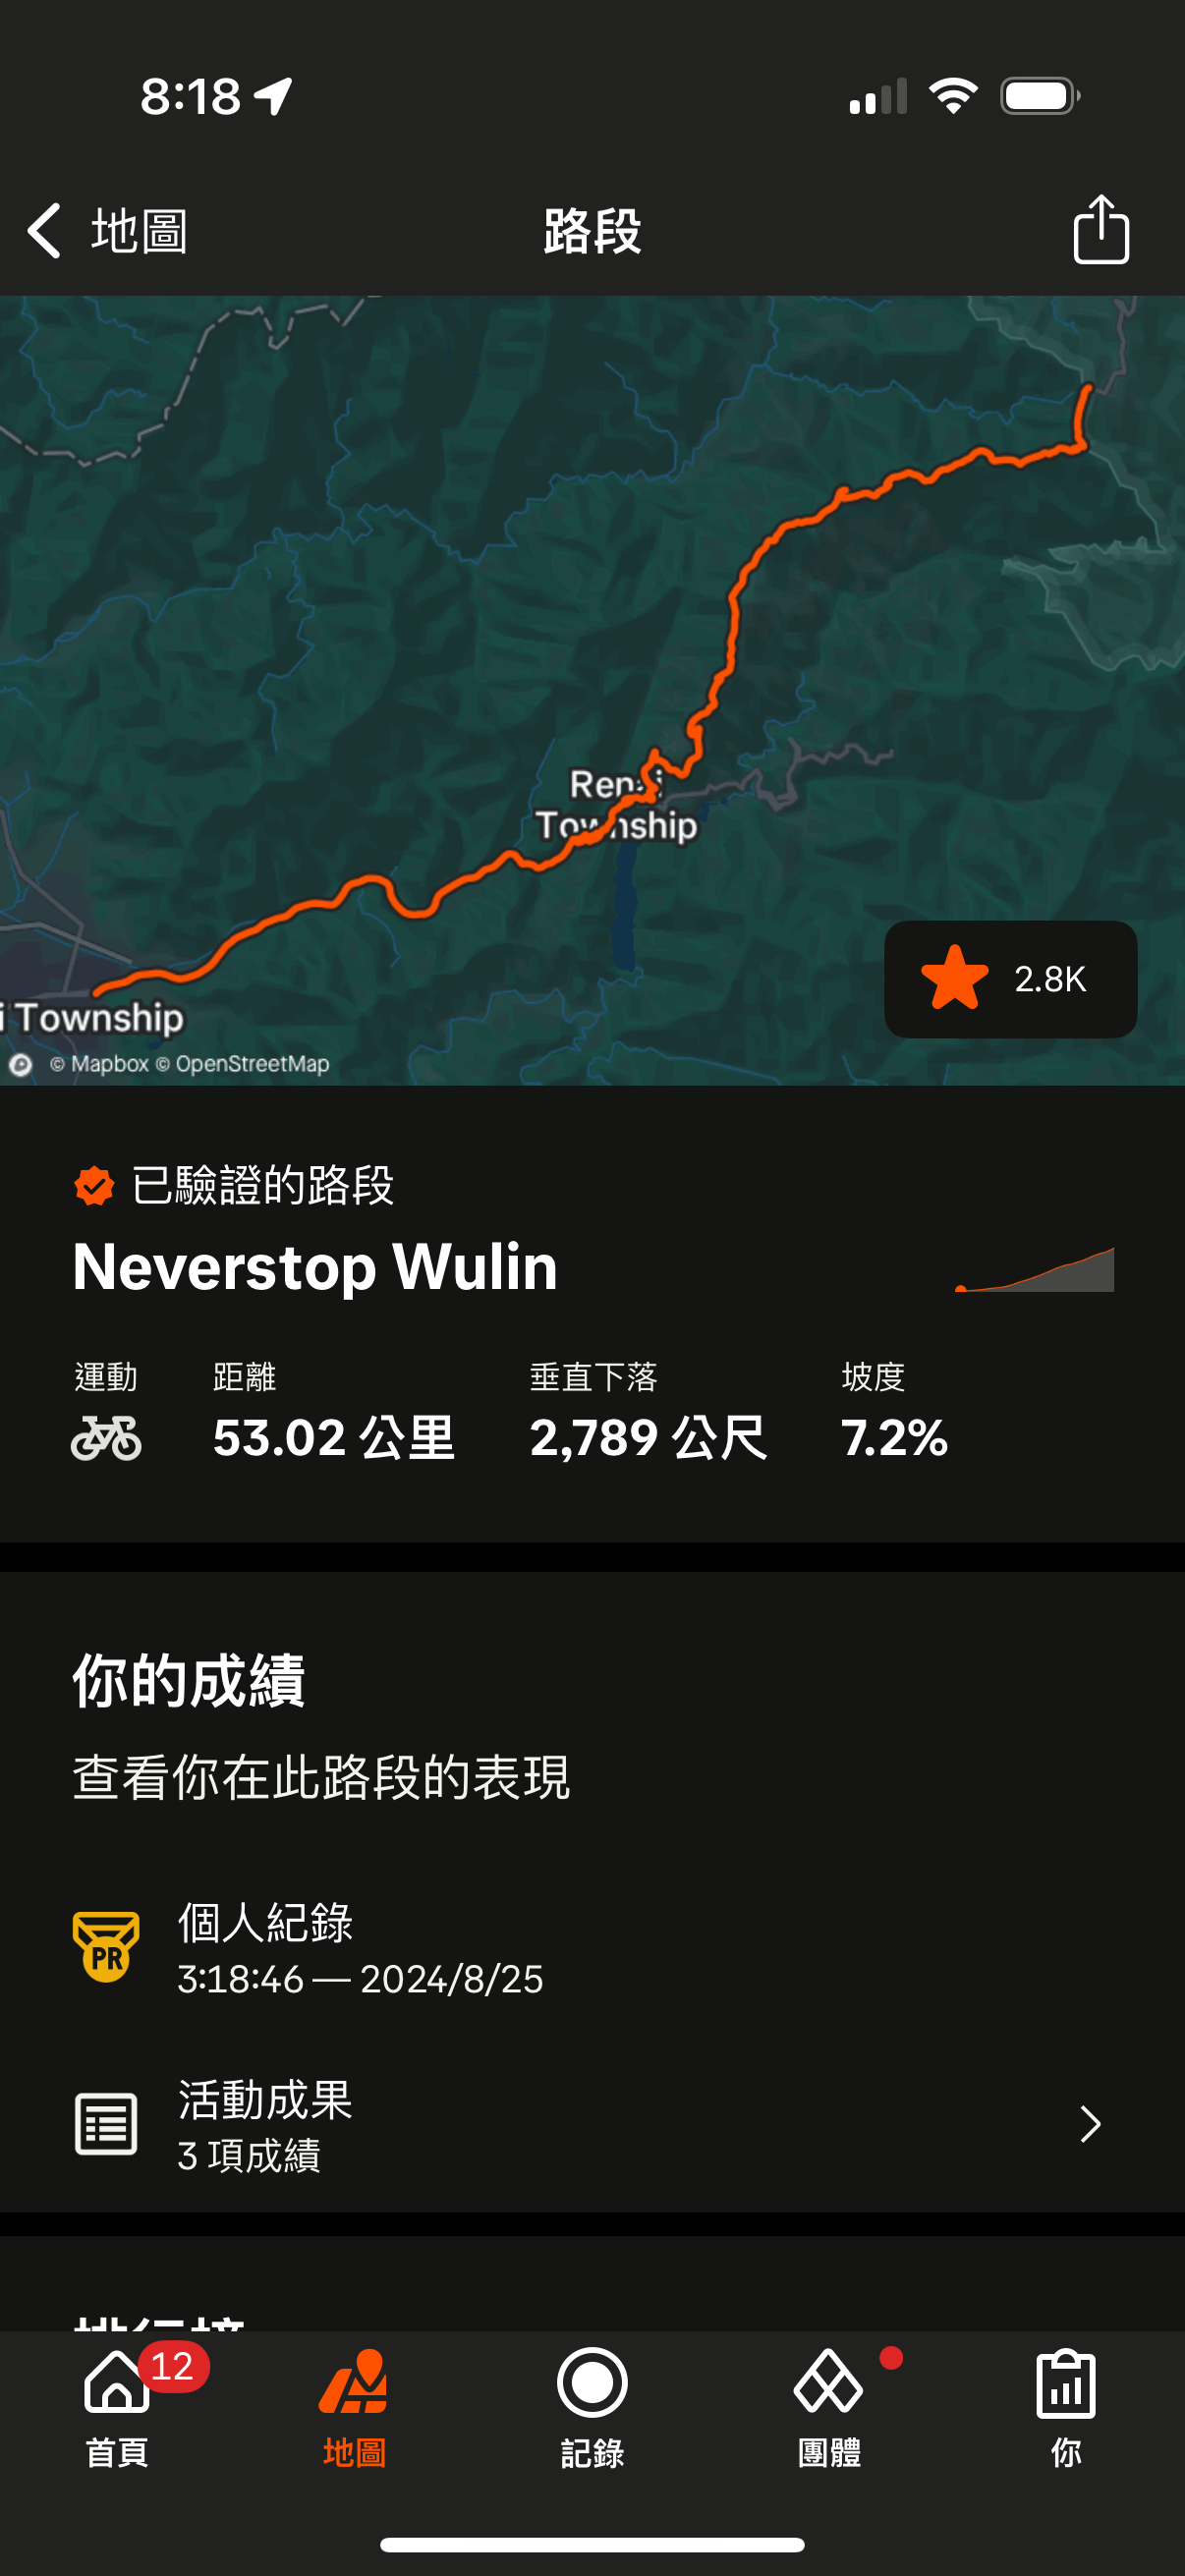
\includegraphics[height=5cm]{wulingSegment.png}
\end{itemize}
\end{frame}

\begin{frame}{名詞}
\begin{itemize}
\item PR (Personal Record) / PB (Personal Best) :個人(最佳)紀錄
\item 皇冠:在一個路段拿到總排第一名 / 女子第一名,拿到皇冠的稱為登山王 (KOM, King of Mountain) / 登山女王 (QOM, Queen of Mountain)
\item 獎盃:在一個路段拿到總排前十名 / 女子前十名
\item Local Legend: 九十天內在一個路段騎過最多次的人
\item 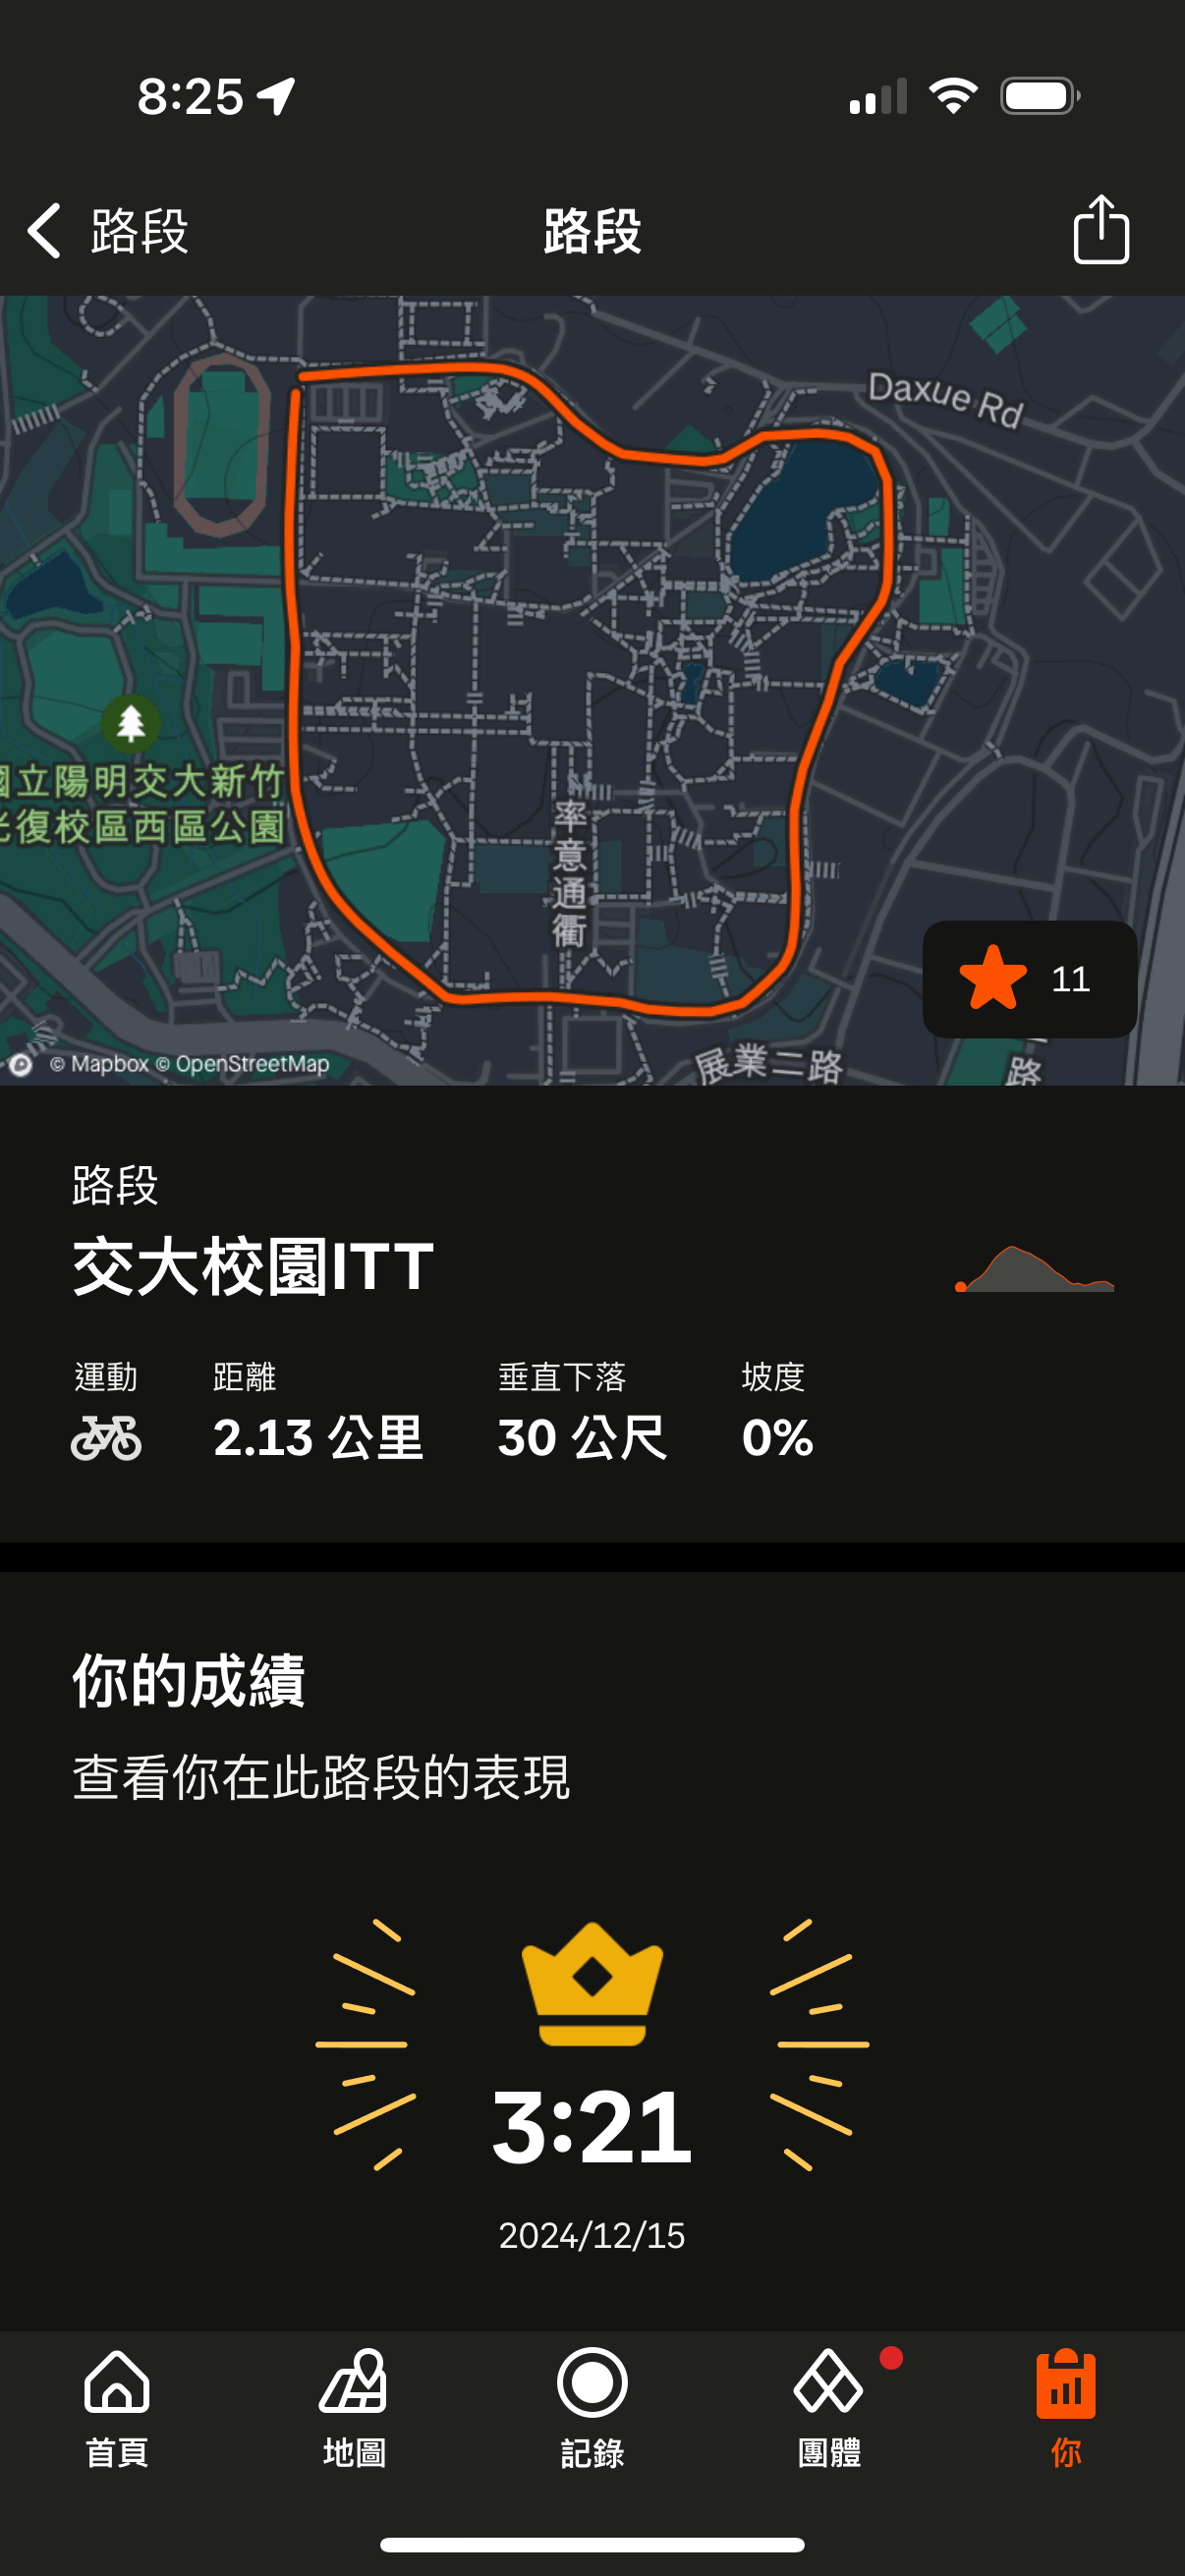
\includegraphics[height=5cm]{KOM.png}
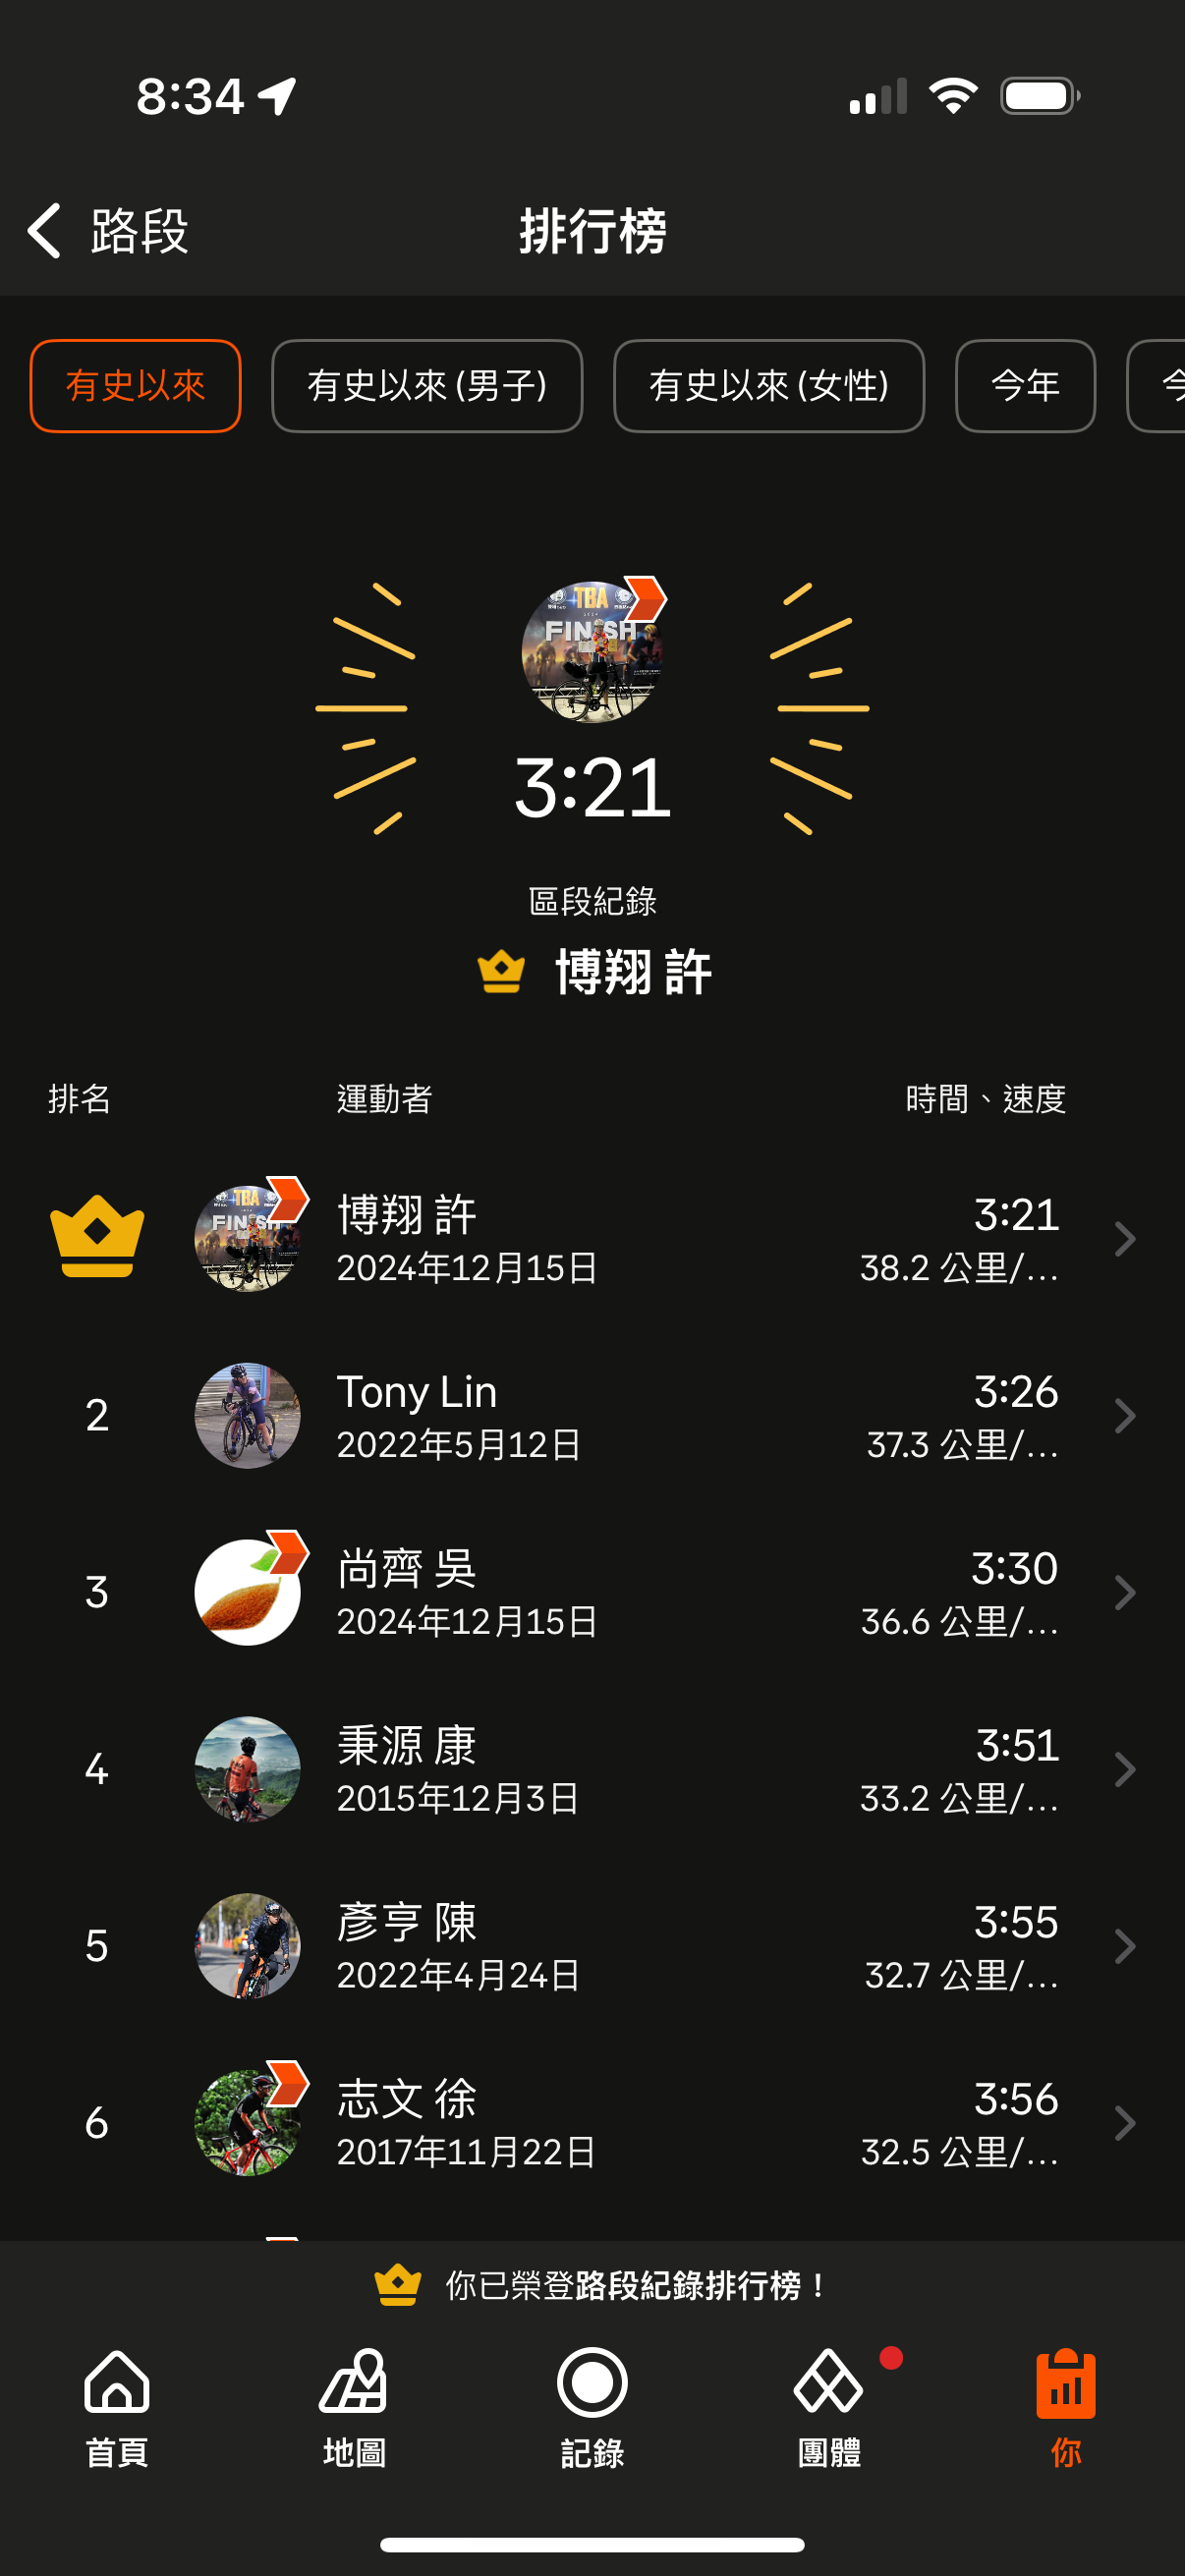
\includegraphics[height=5cm]{KOM2.png}
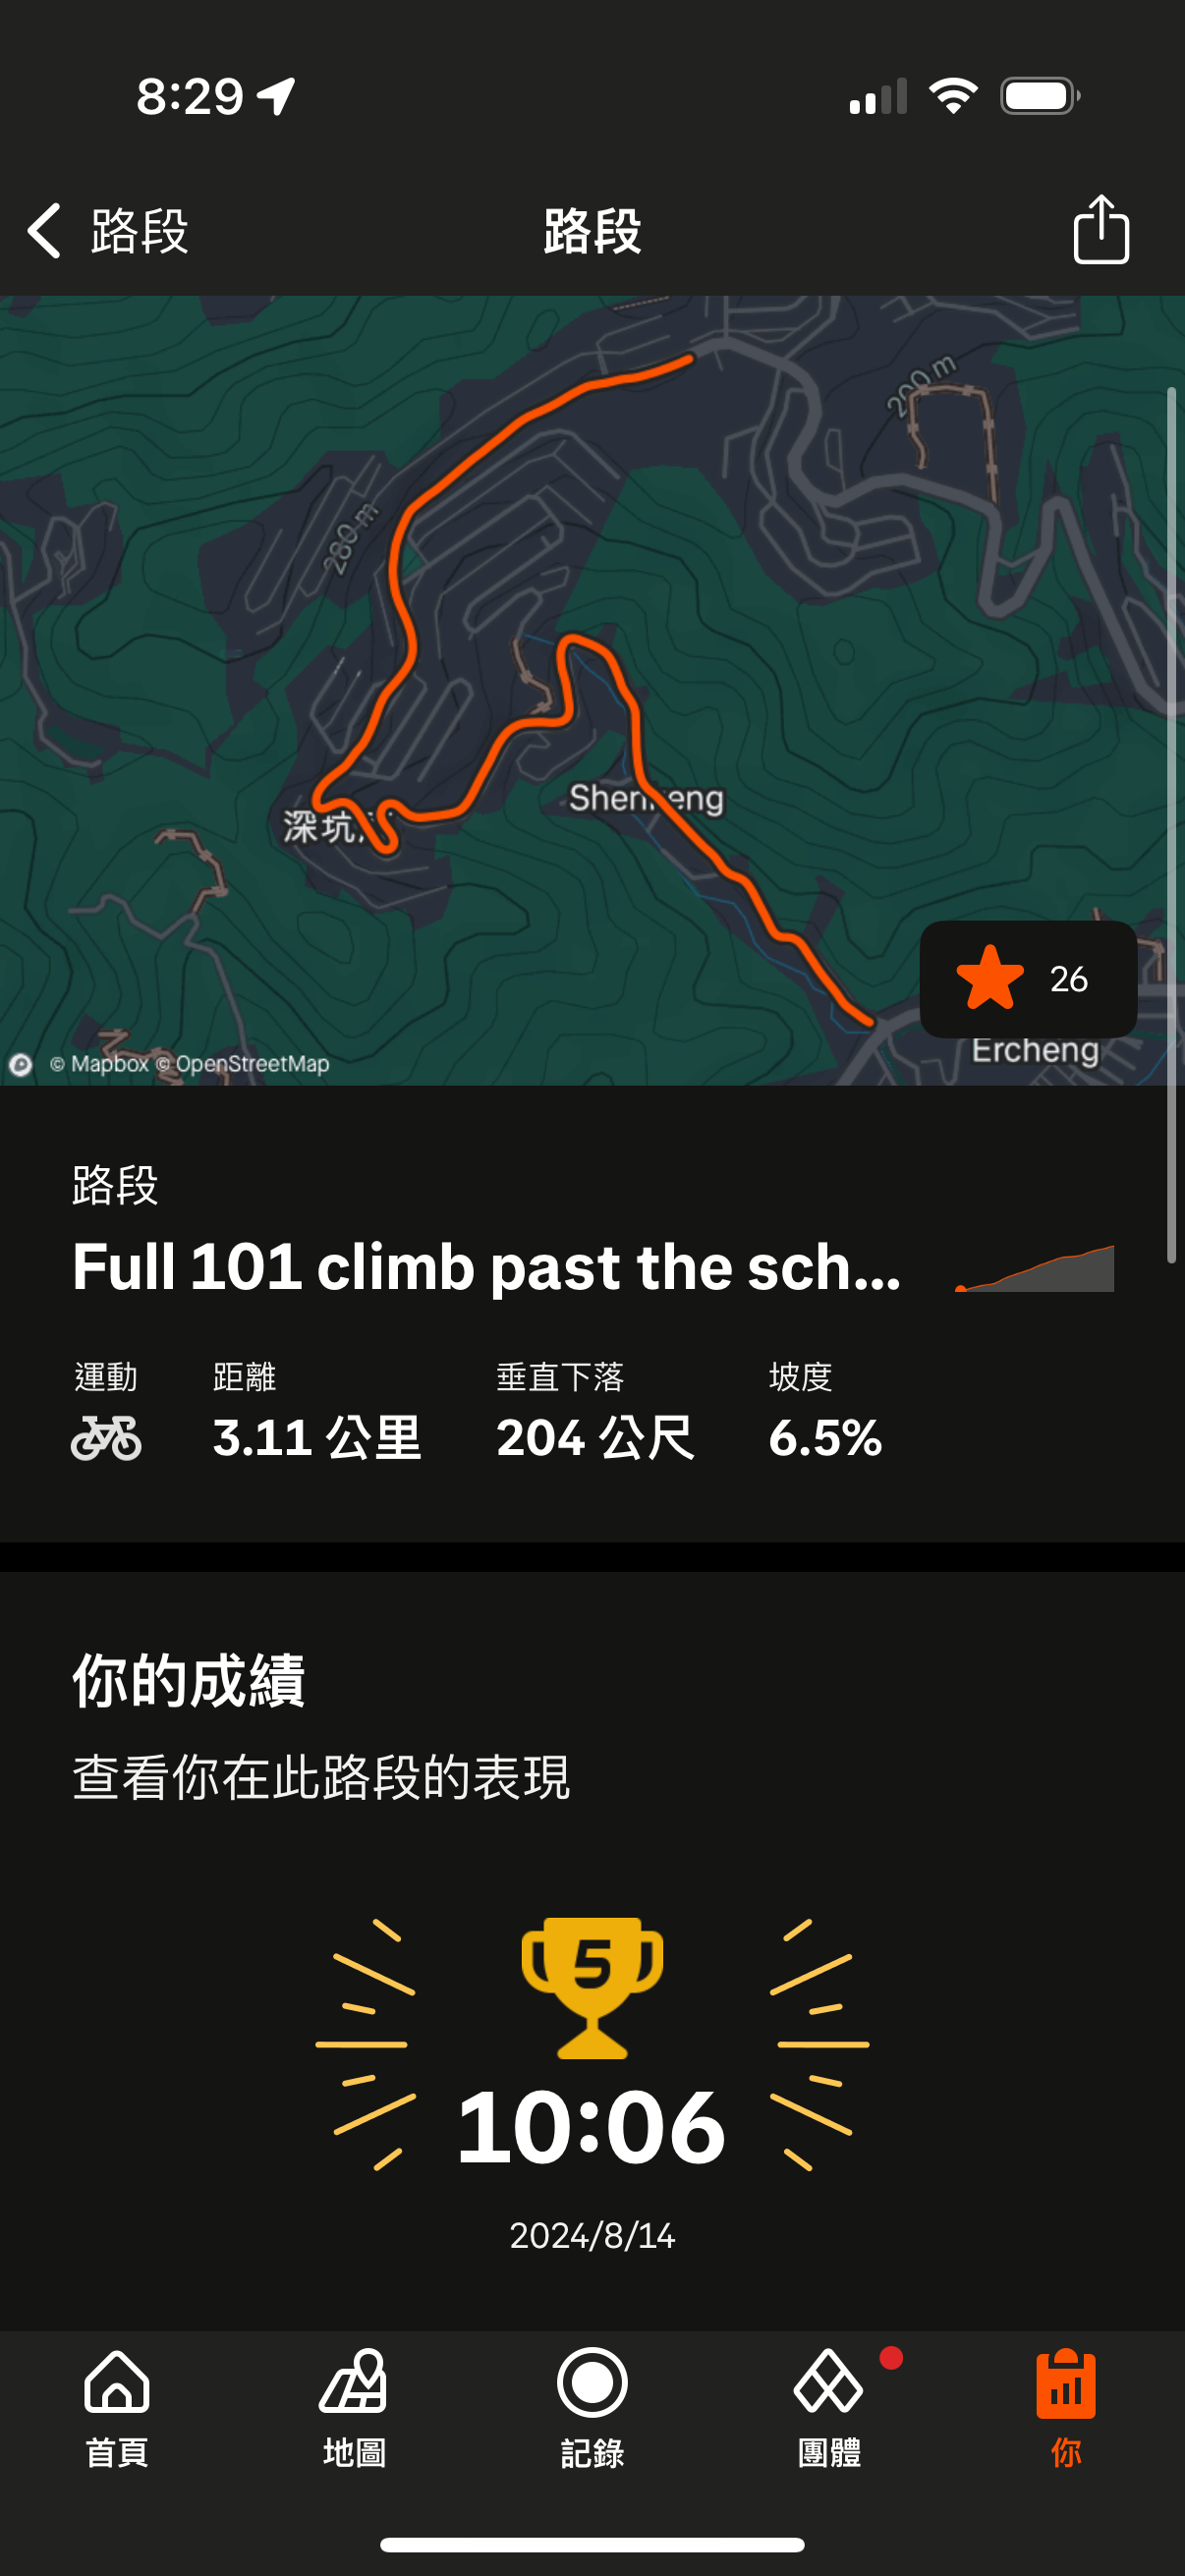
\includegraphics[height=5cm]{trophy.png}
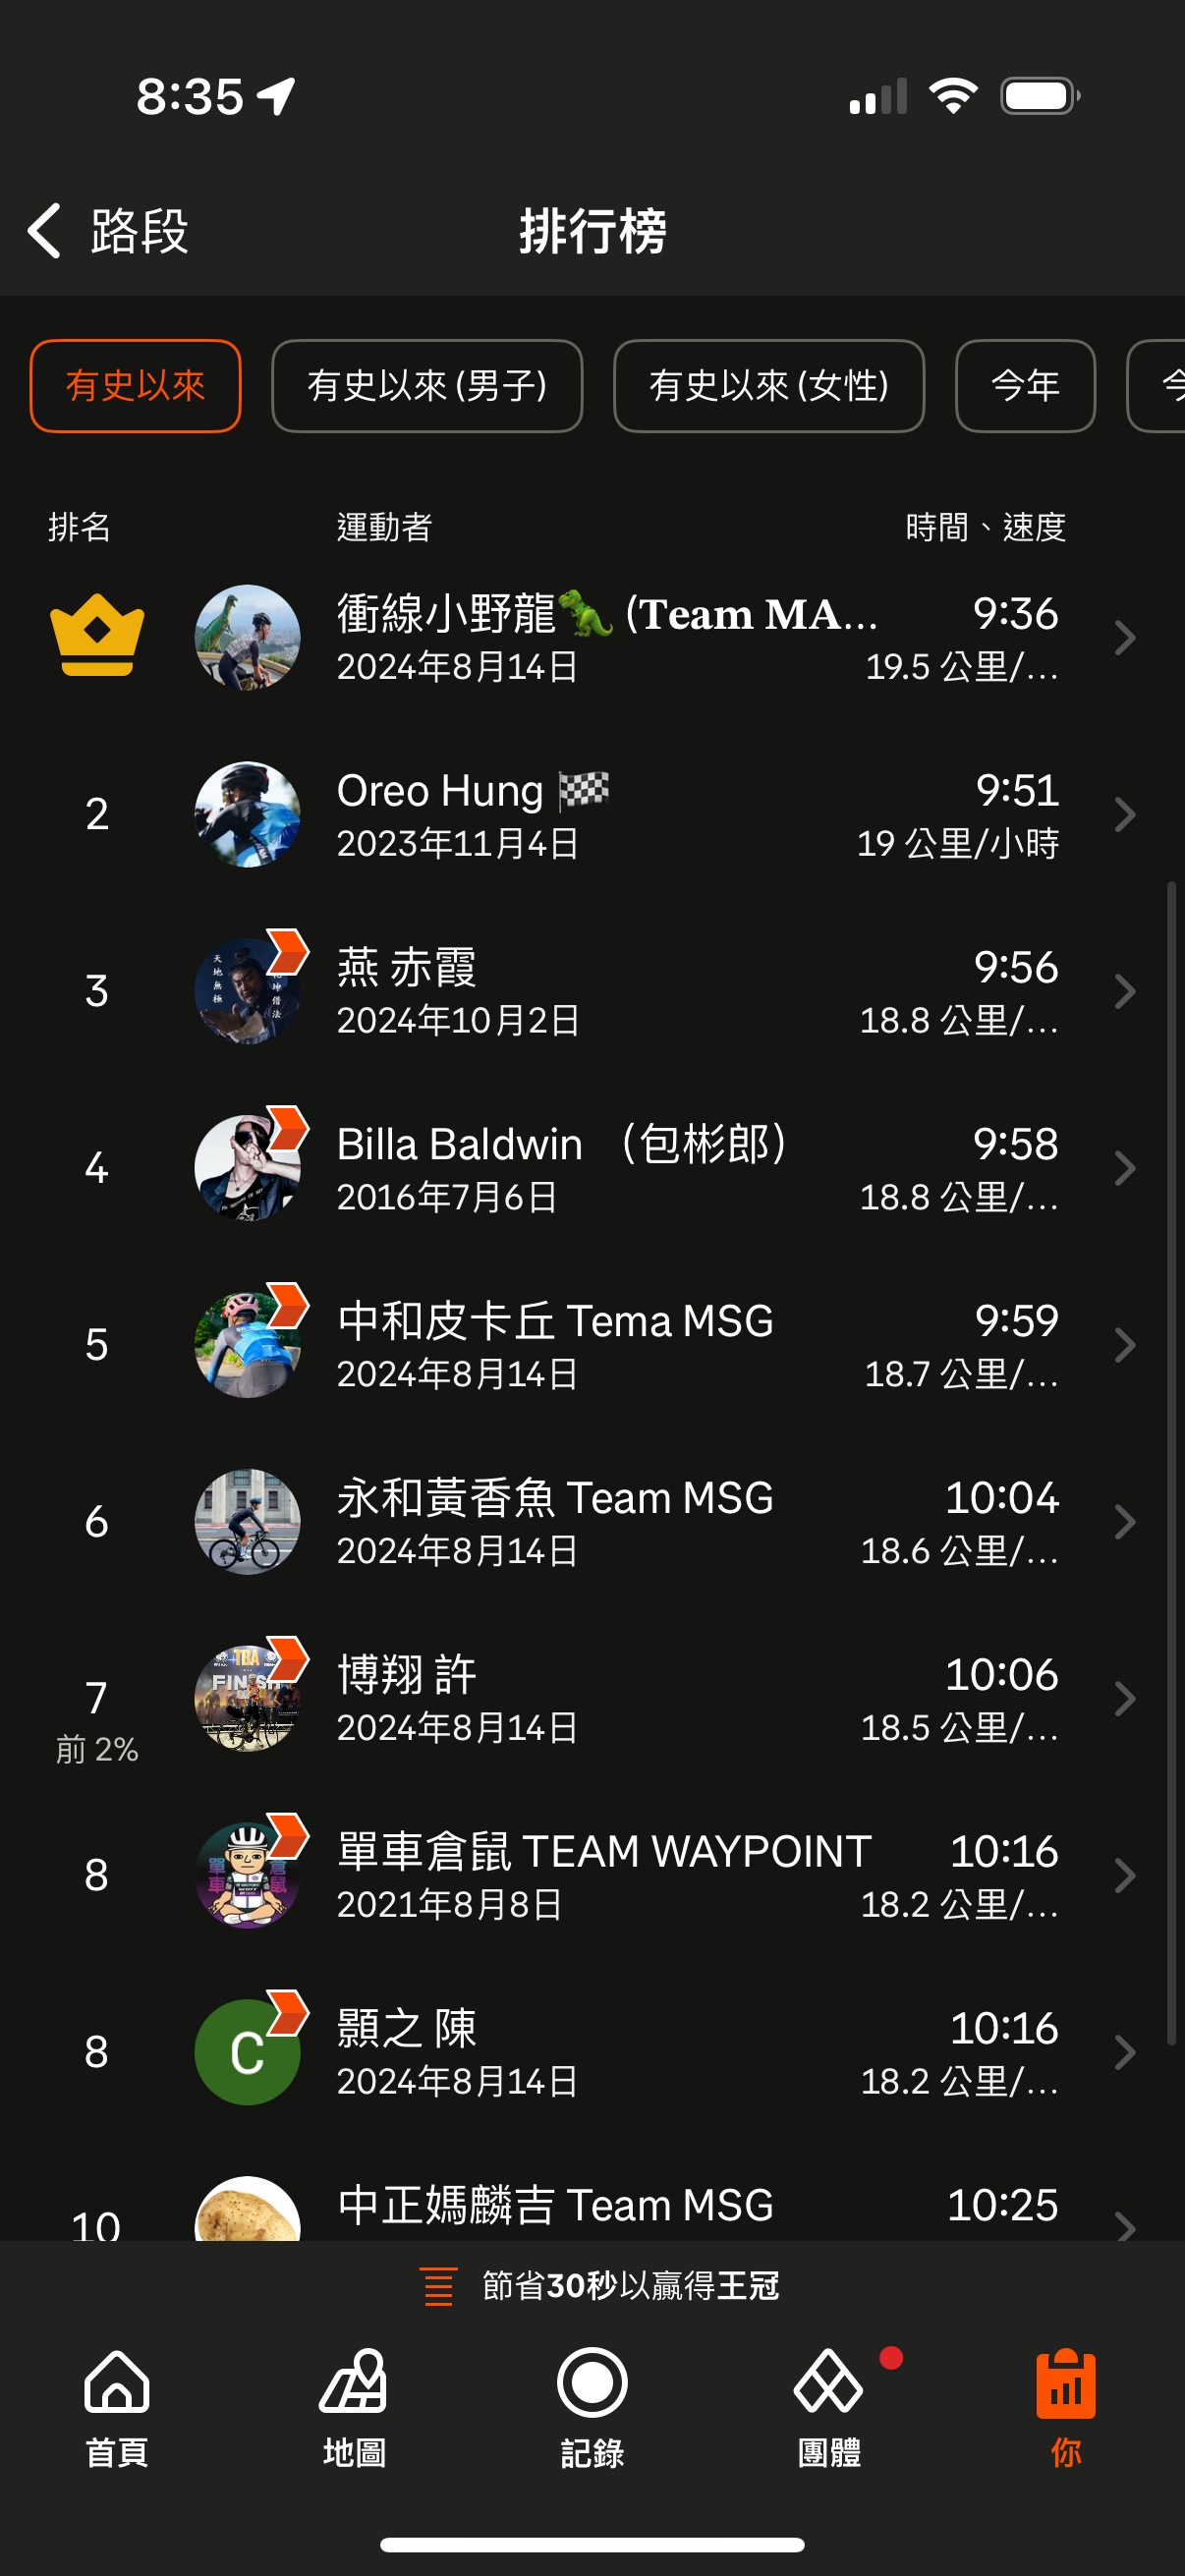
\includegraphics[height=5cm]{trophy2.png}
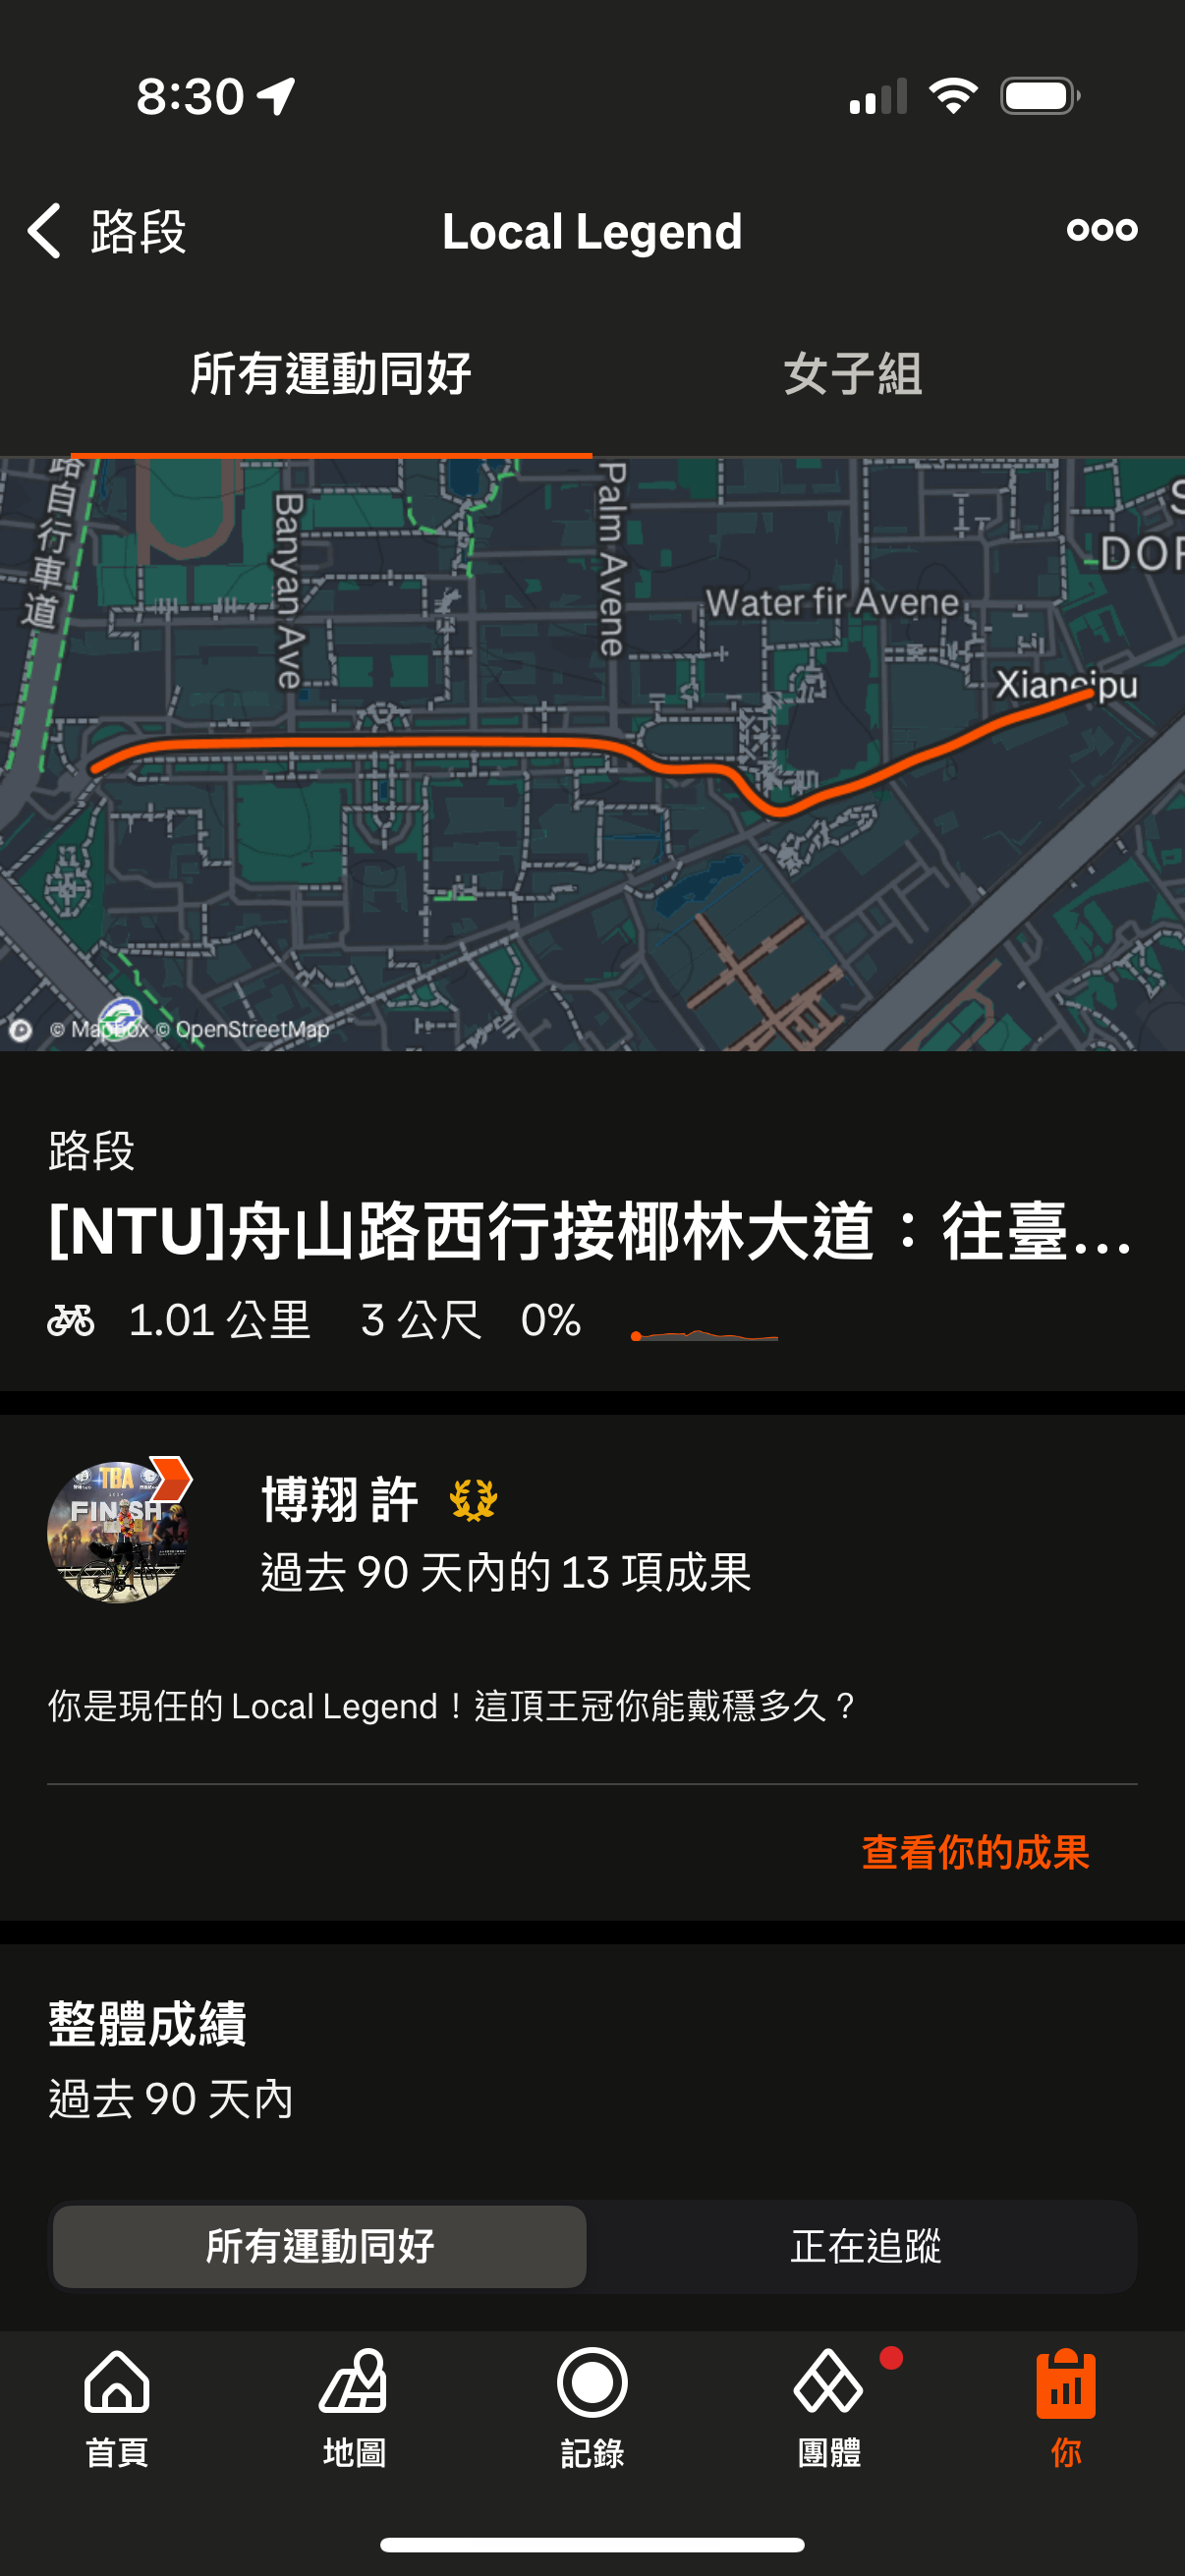
\includegraphics[height=5cm]{localLegend.png}
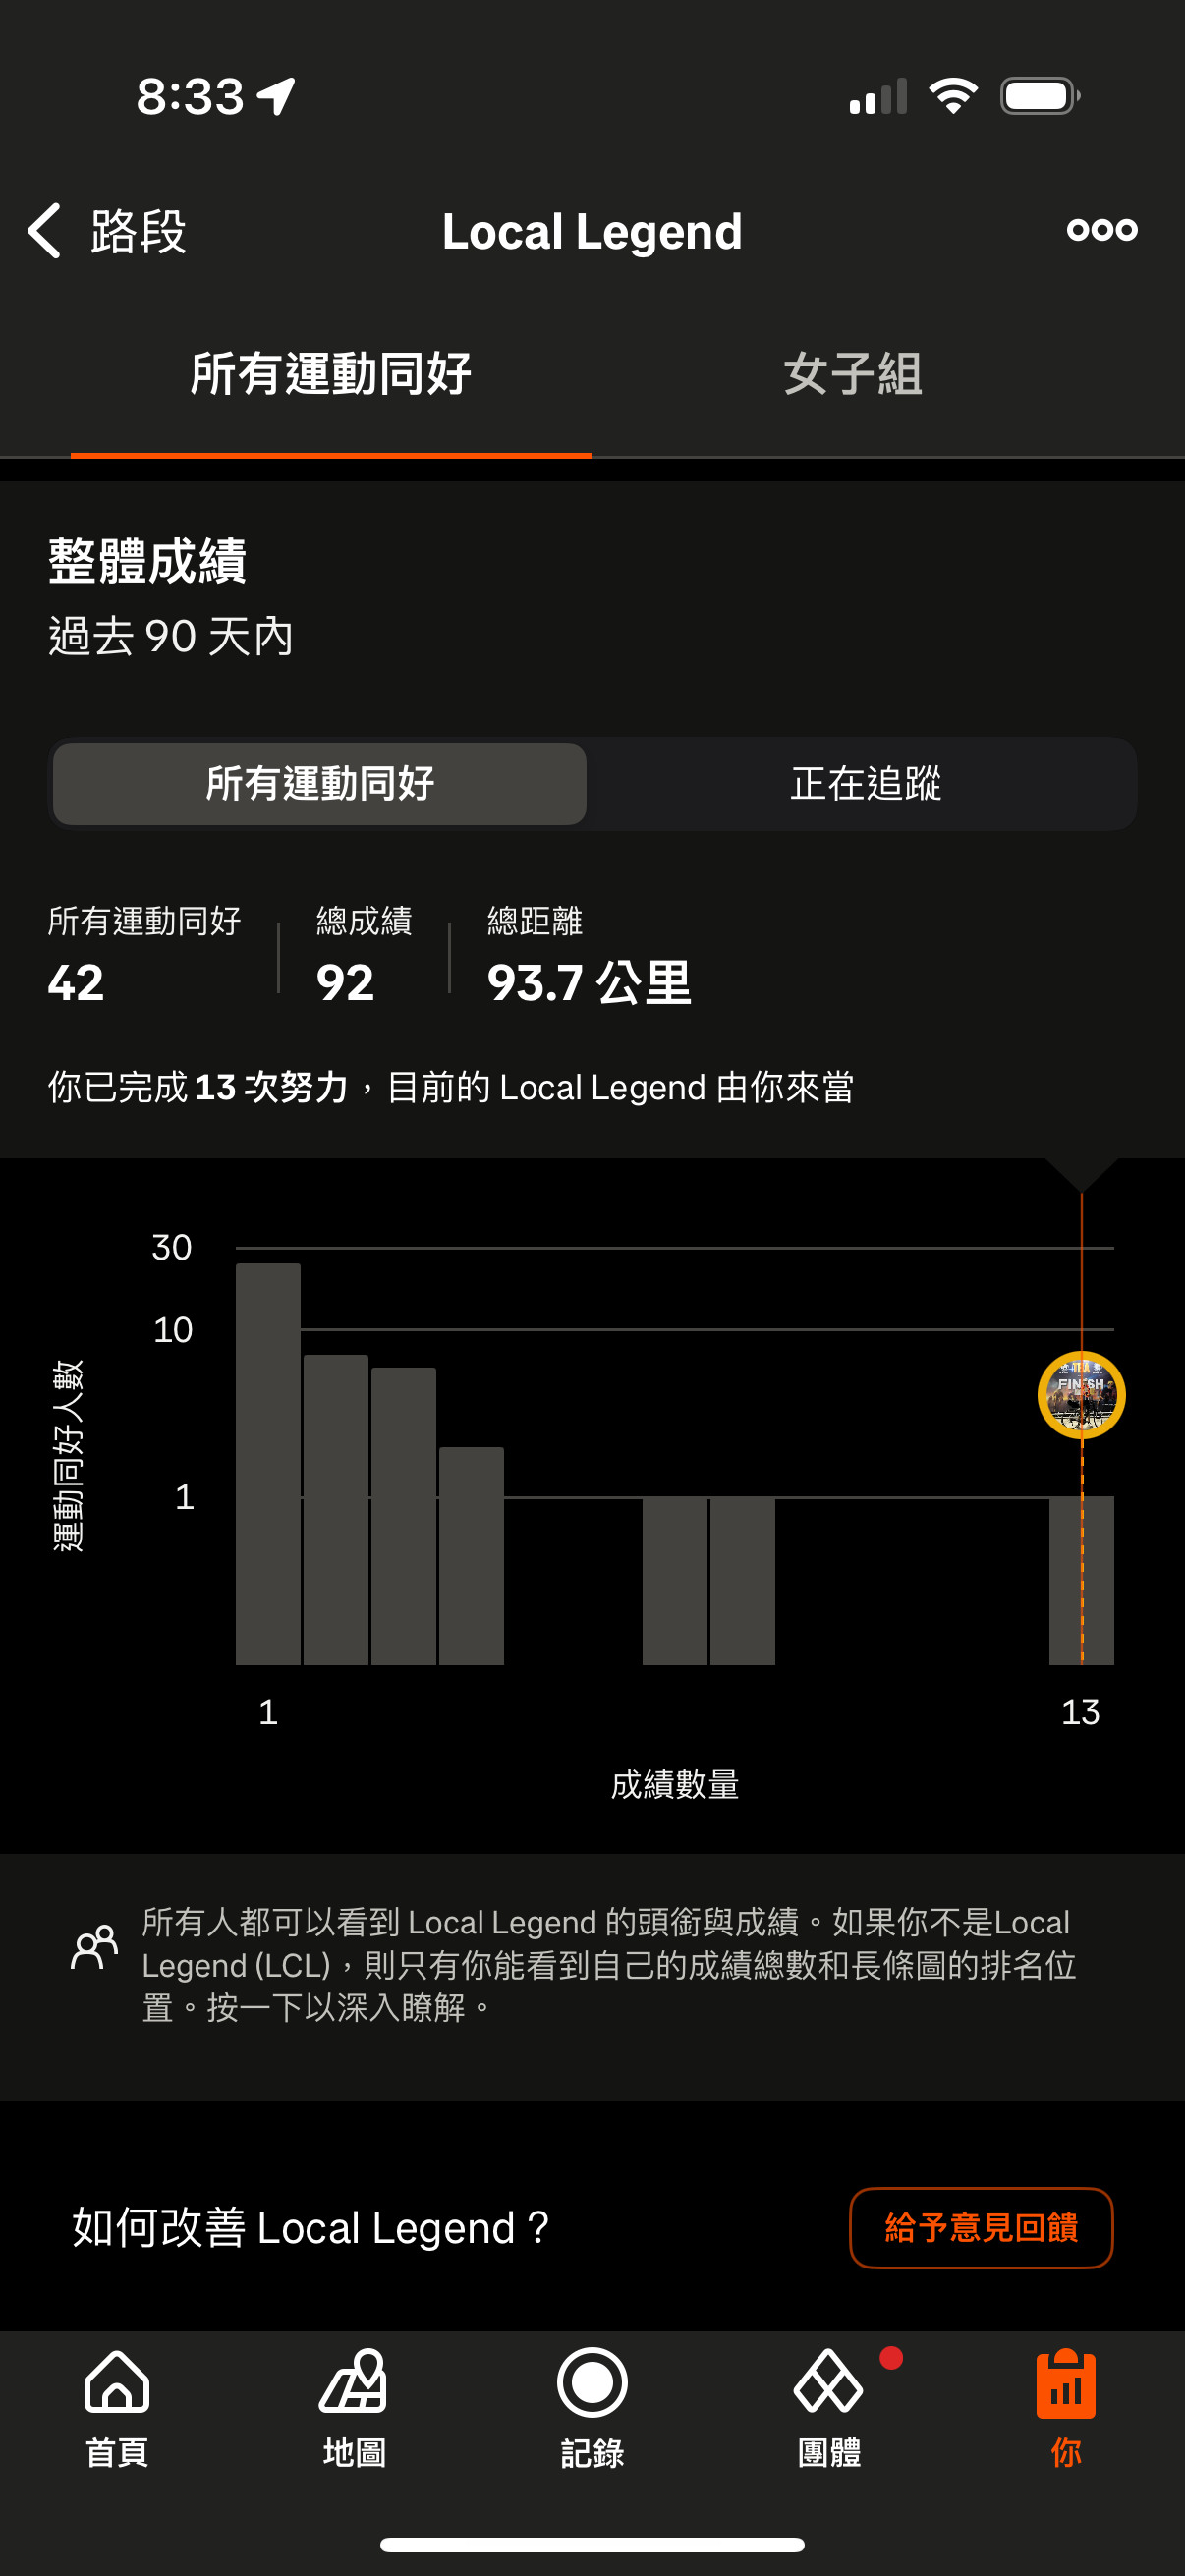
\includegraphics[height=5cm]{localLegend2.png}
\end{itemize}
\end{frame}

\begin{frame}{排名}
\begin{multicols}{2}
\begin{itemize}
\item 年齡:依年齡分組排名(比如我在20至24歲組)
\item 體重:依體重分組排名(比如我在55至64公斤組)
\item 今年:當年度的排名
\item 今天:當天的排名,如果不是太熱門的路段,通常可以在團騎拿來看各自的速度
\item	正在追蹤:你跟你正在追蹤的人之間的排名,比如如果追蹤新店奧特曼,那可能在大部分的路段名次都會往後一名
\item 社團:可以看自己的社內排名
\newpage
\item 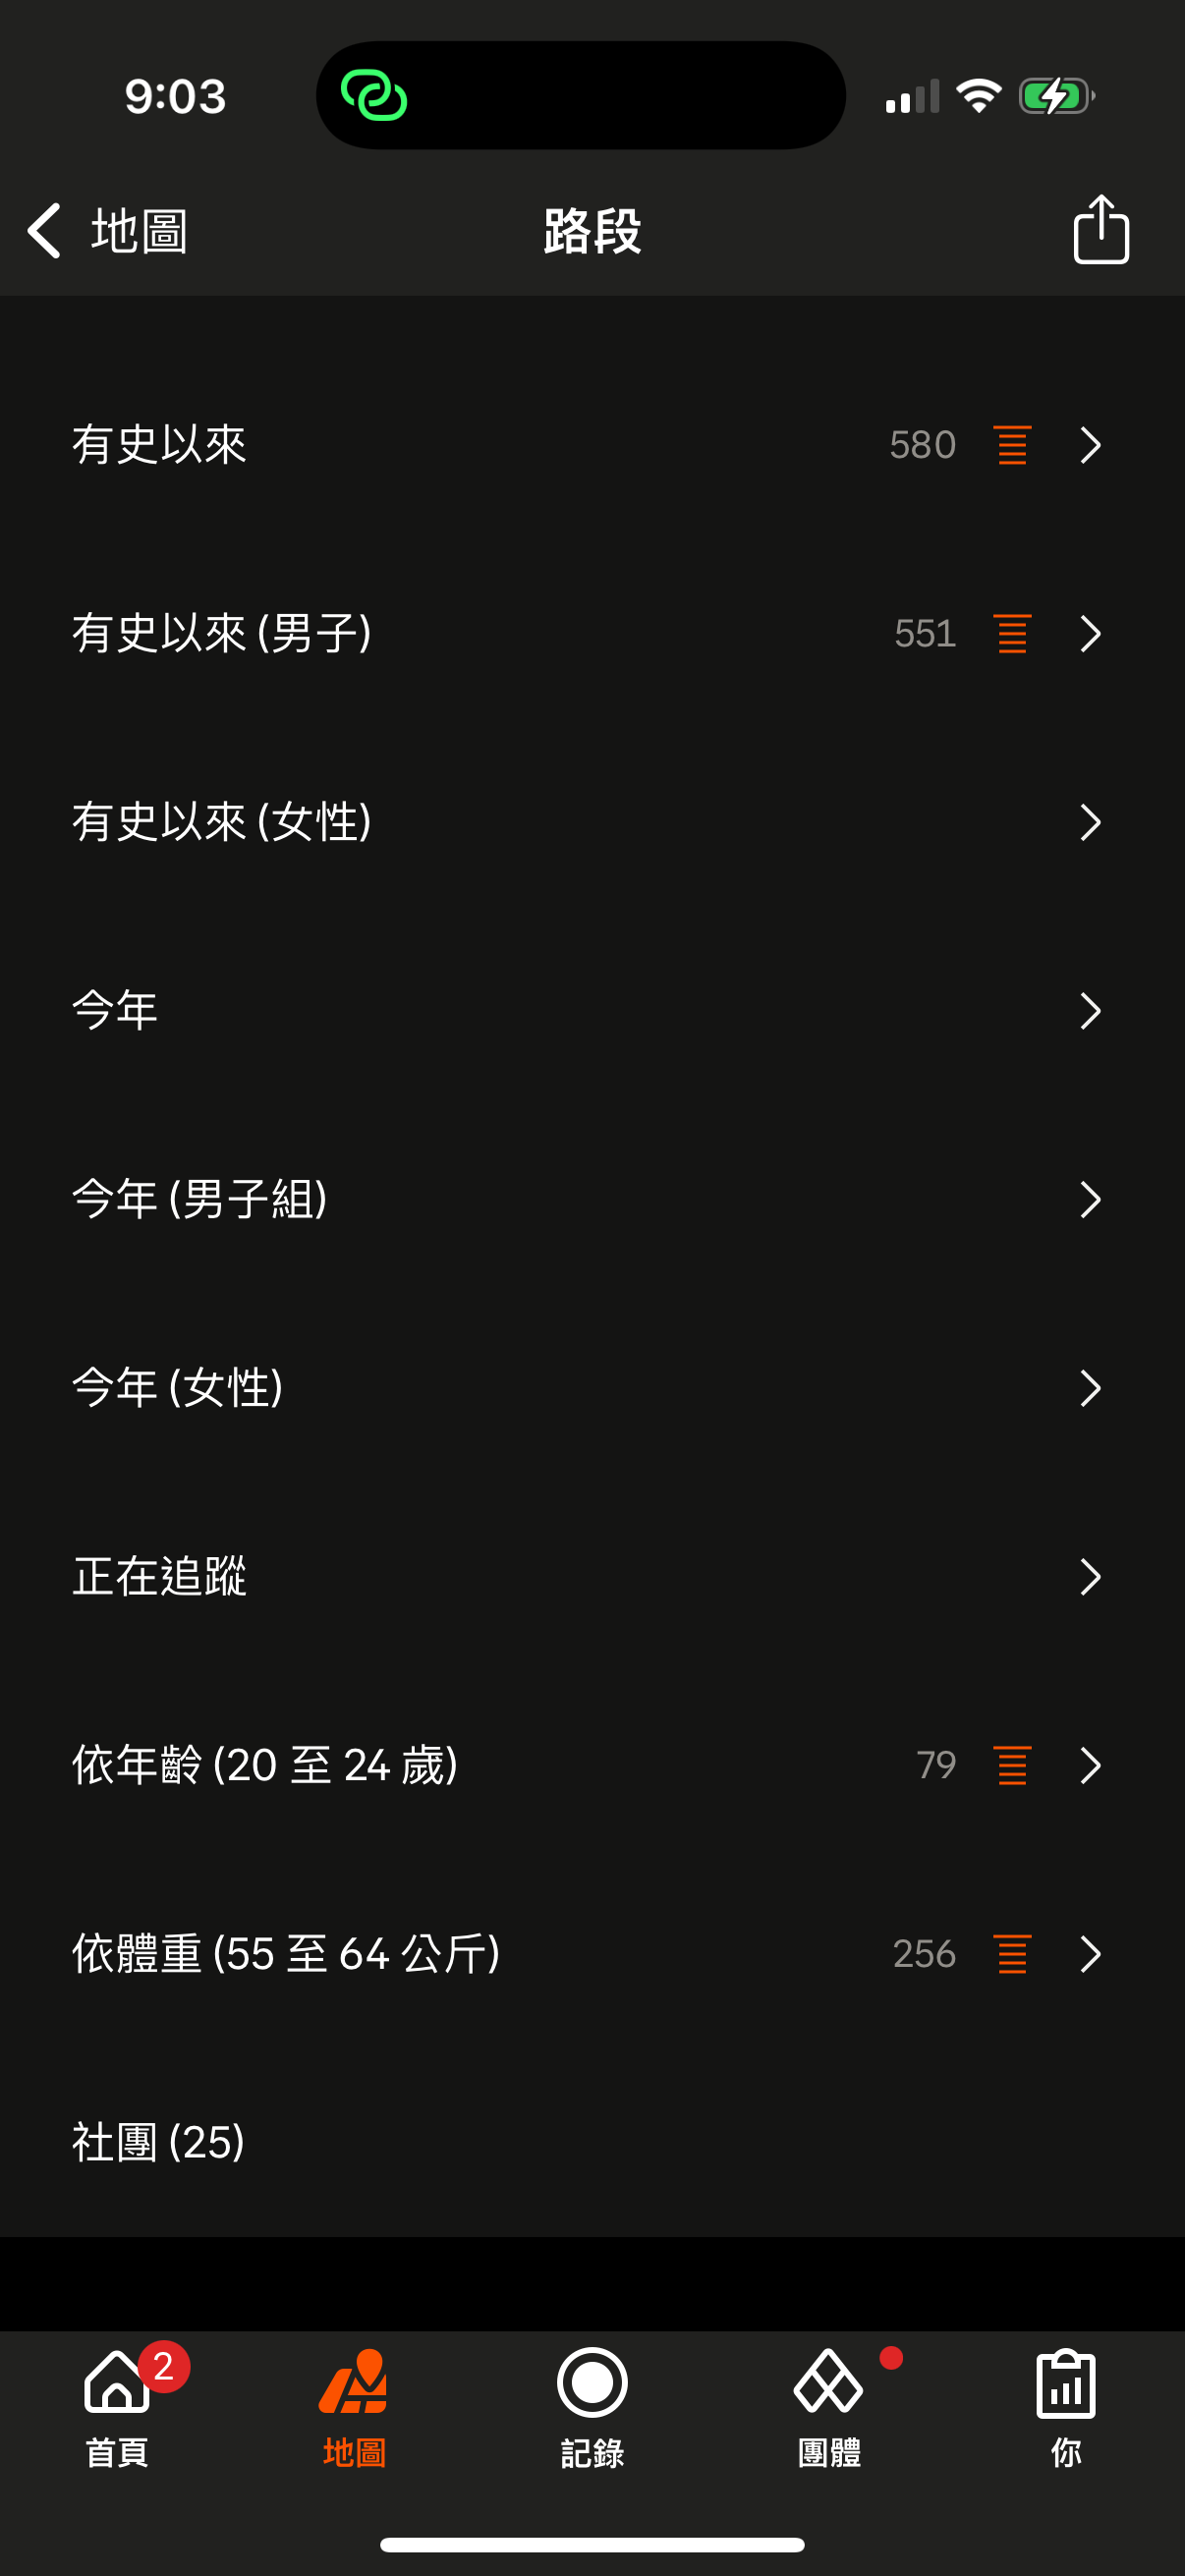
\includegraphics[height=7cm]{rank.png}
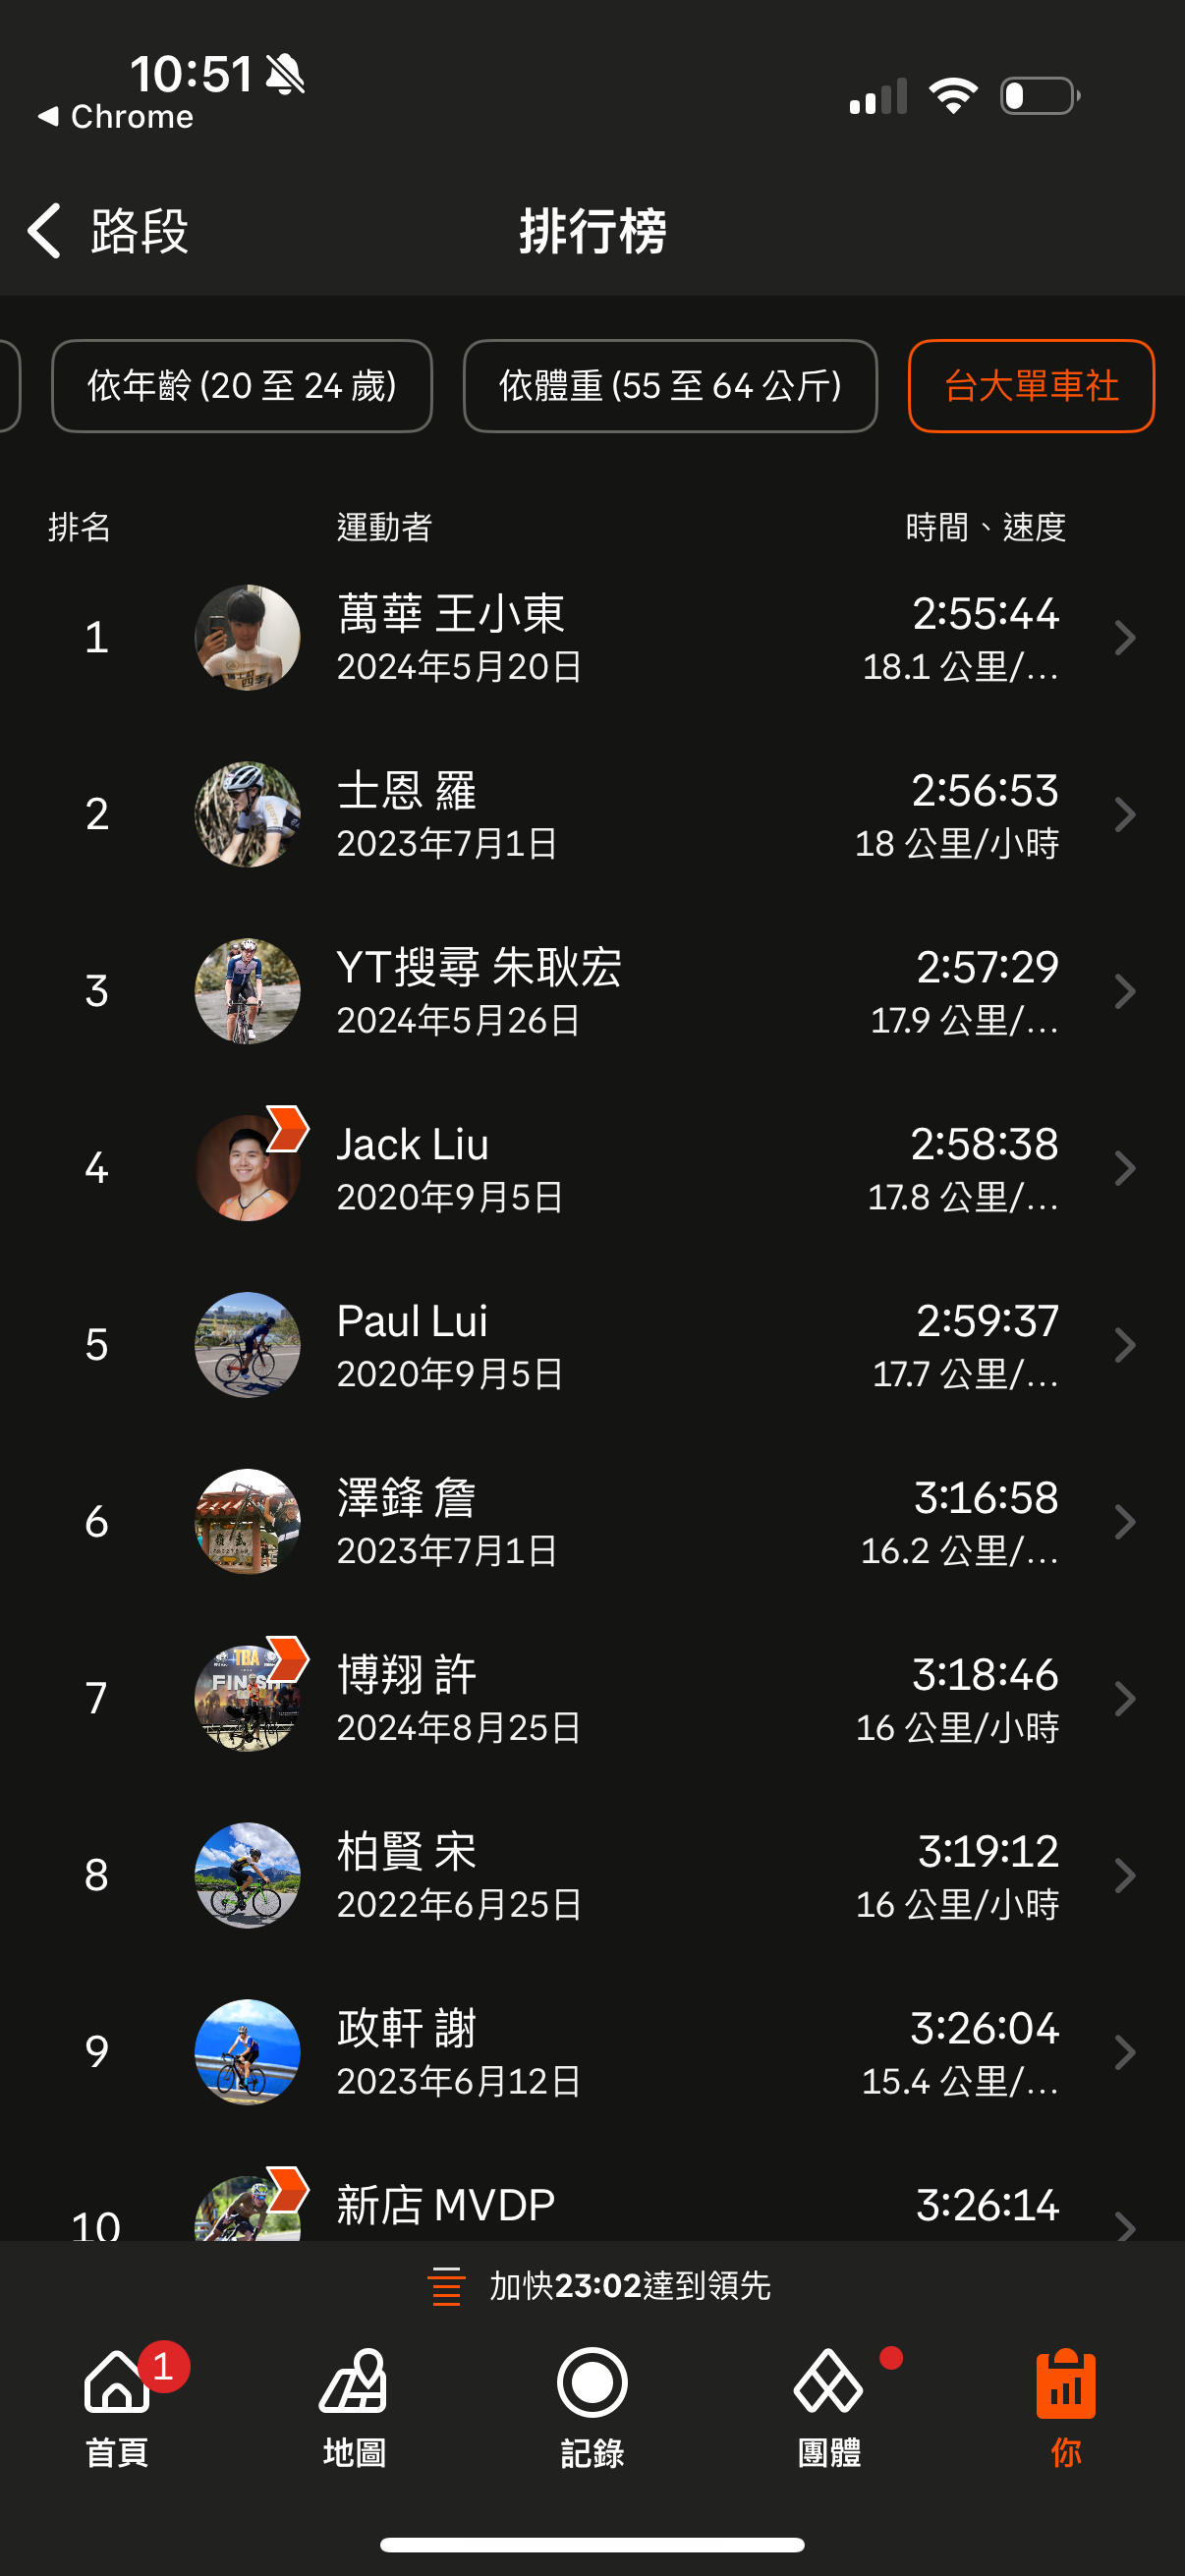
\includegraphics[height=7cm]{rank2.png}
\end{itemize}
\end{multicols}
\end{frame}

\begin{frame}{計時原理}
\begin{multicols}{2}
\begin{itemize}
\item 路段時間$=$通過終點的時間$-$通過起點的時間
\item 通過起/終點判定
\begin{itemize}
\item 活動:由一堆點(通常一秒一個)組成的一條折線
\item 通過起/終點:這些點與起/終點距離的 local minimum ,也就是在一個區間之內與起/終點距離最近的點
\end{itemize}
\item 計時狀態:通過起點之後,依序抵達路段中的各個點,並且未偏離路段太遠
\item 計時流程
\begin{itemize}
\item 通過起點
\item 計時狀態
\item 通過終點
\end{itemize}
\newpage
\pause
\item 你以為的路段
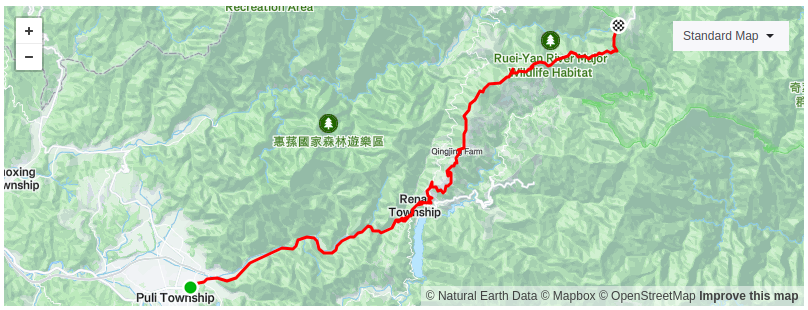
\includegraphics[width=5.5cm]{wulingMap.png}
\item 實際上的路段
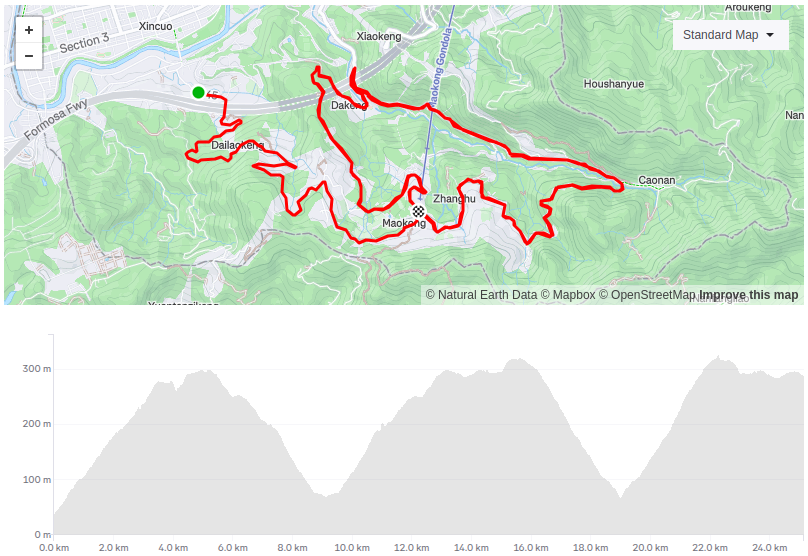
\includegraphics[width=5.5cm]{maokong3pMap.png}
\end{itemize}
\end{multicols}
\end{frame}

\newcommand{\yes}[1]{\alt<2>{\textcolor{red}{#1}}{\textcolor{black}{#1}}}
\newcommand{\maybe}[1]{\alt<2>{\textcolor{orange}{#1}}{\textcolor{black}{#1}}}

\begin{frame}[fragile]{如何避免計時失敗}
\begin{itemize}
\item 計時失敗: Strava 上的路段時間明顯跟騎的時間不一樣
\item 下列哪些情況容易造成計時失敗?
\begin{enumerate}[A]
\item \yes{在起點休息了一會之後直接上山(例如在萊爾富三芝天涯店休息,休完之後直接計時巴拉卡)}
\item \yes{計時完直接停在終點等待其他隊友(例如爬完助航站直接停在旁邊拍大屯山風景)}
\item \yes{計時到一半折返找隊友}
\item 計時途中停在路邊休息
\item \yes{計時途中岔出去其他地方再回來(例如騎冷水坑途中跑去平菁街看櫻花)}
\item \yes{騎不同條路(例如要計時貓空指南線但騎草湳那條路)}
\item \href{https://www.instagram.com/reel/C5tCGSeyQNI/?utm_source=ig_web_button_share_sheet}{邊計時邊跳舞}
\item \maybe{闖紅燈}
\item \yes{過山洞}
\item \maybe{計時中遇到狗}
\item 計時中搭車
\item \yes{計時中按到暫停}
\end{enumerate}
\end{itemize}
\end{frame}

\begin{frame}{如何避免計時失敗}
\begin{itemize}
\item \sout{在起點休息了一會之後直接上山}\\
出發前先離開起點夠遠的一段距離,再重新進入起點重新開始計時
\item \sout{計時完直接停在終點等待其他隊友}\\
抵達終點之後先離開終點夠遠的一段距離,以確保計時結束
\item \sout{計時到一半折返找隊友}\\
折返時停錶,回到折返點再按錶繼續
\item \sout{計時途中岔出去其他地方再回來}\\
岔出去時停錶,回到出去的點再按錶繼續
\item \sout{騎不同條路}\\
基本上沒救
\item \sout{過山洞}\\
基本上沒救,所以創路段會盡量避免經過過長的山洞
\item \sout{計時中按到暫停}\\
回到按暫停的點按錶繼續計時
\end{itemize}
\end{frame}

\begin{frame}{計時失敗補救}
\begin{itemize}
\item 編輯/裁切活動,重新上傳
\item 把起/終點附近多餘的點拿掉,以讓 Strava 不會把停在那裡休息的點也算進去
\item 把偏離計時路段的點拿掉,以讓 Strava 不會以為你沒在計時
\end{itemize}
\end{frame}

\begin{frame}{有人作弊怎麼辦}
\begin{itemize}
\begin{multicols}{2}
\only<1>{
\item 檢舉他!檢舉完之後他就會從排行榜上消失了。
\item 素材:\href{https://www.strava.com/athletes/117279779}{曹翊}
\item 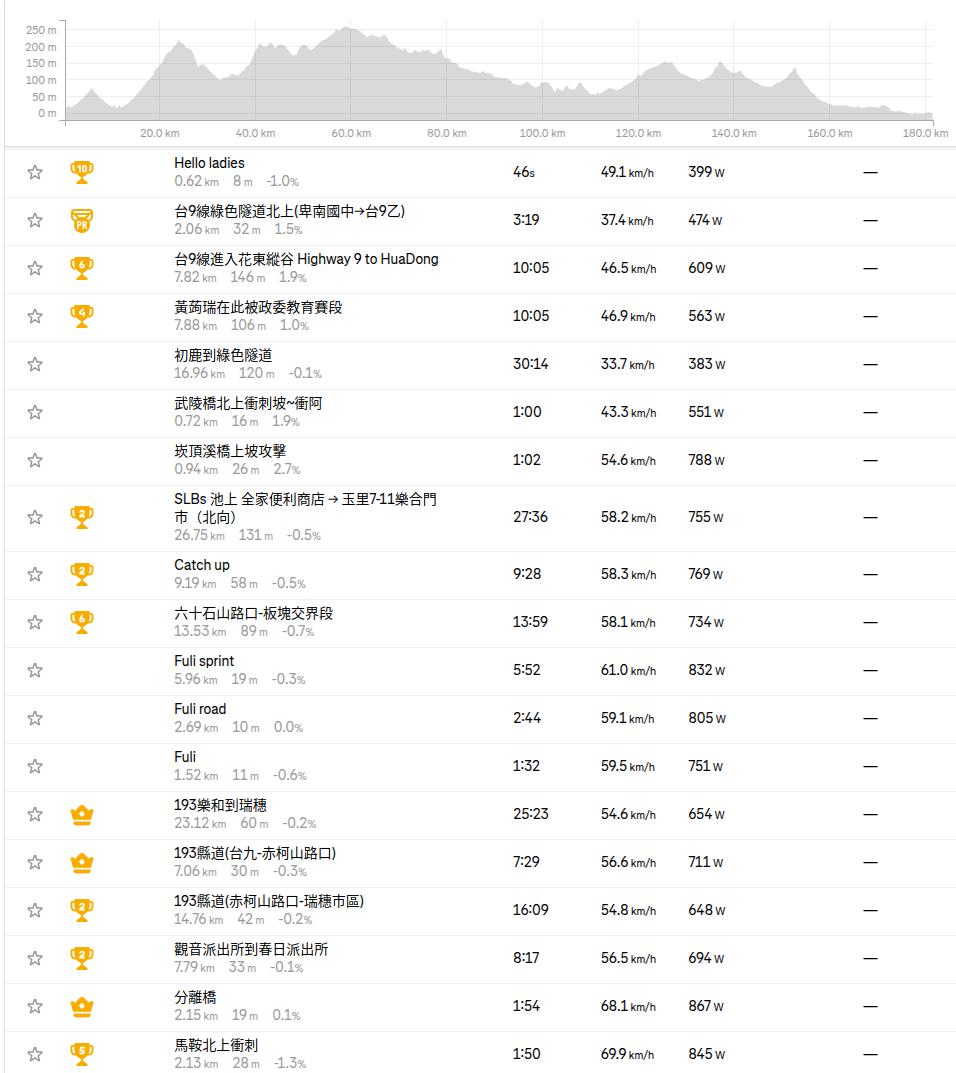
\includegraphics[width=7cm]{flag0.png}
}\only<2>{
\item 點選三個點(Actions)然後選擇 Flag :\\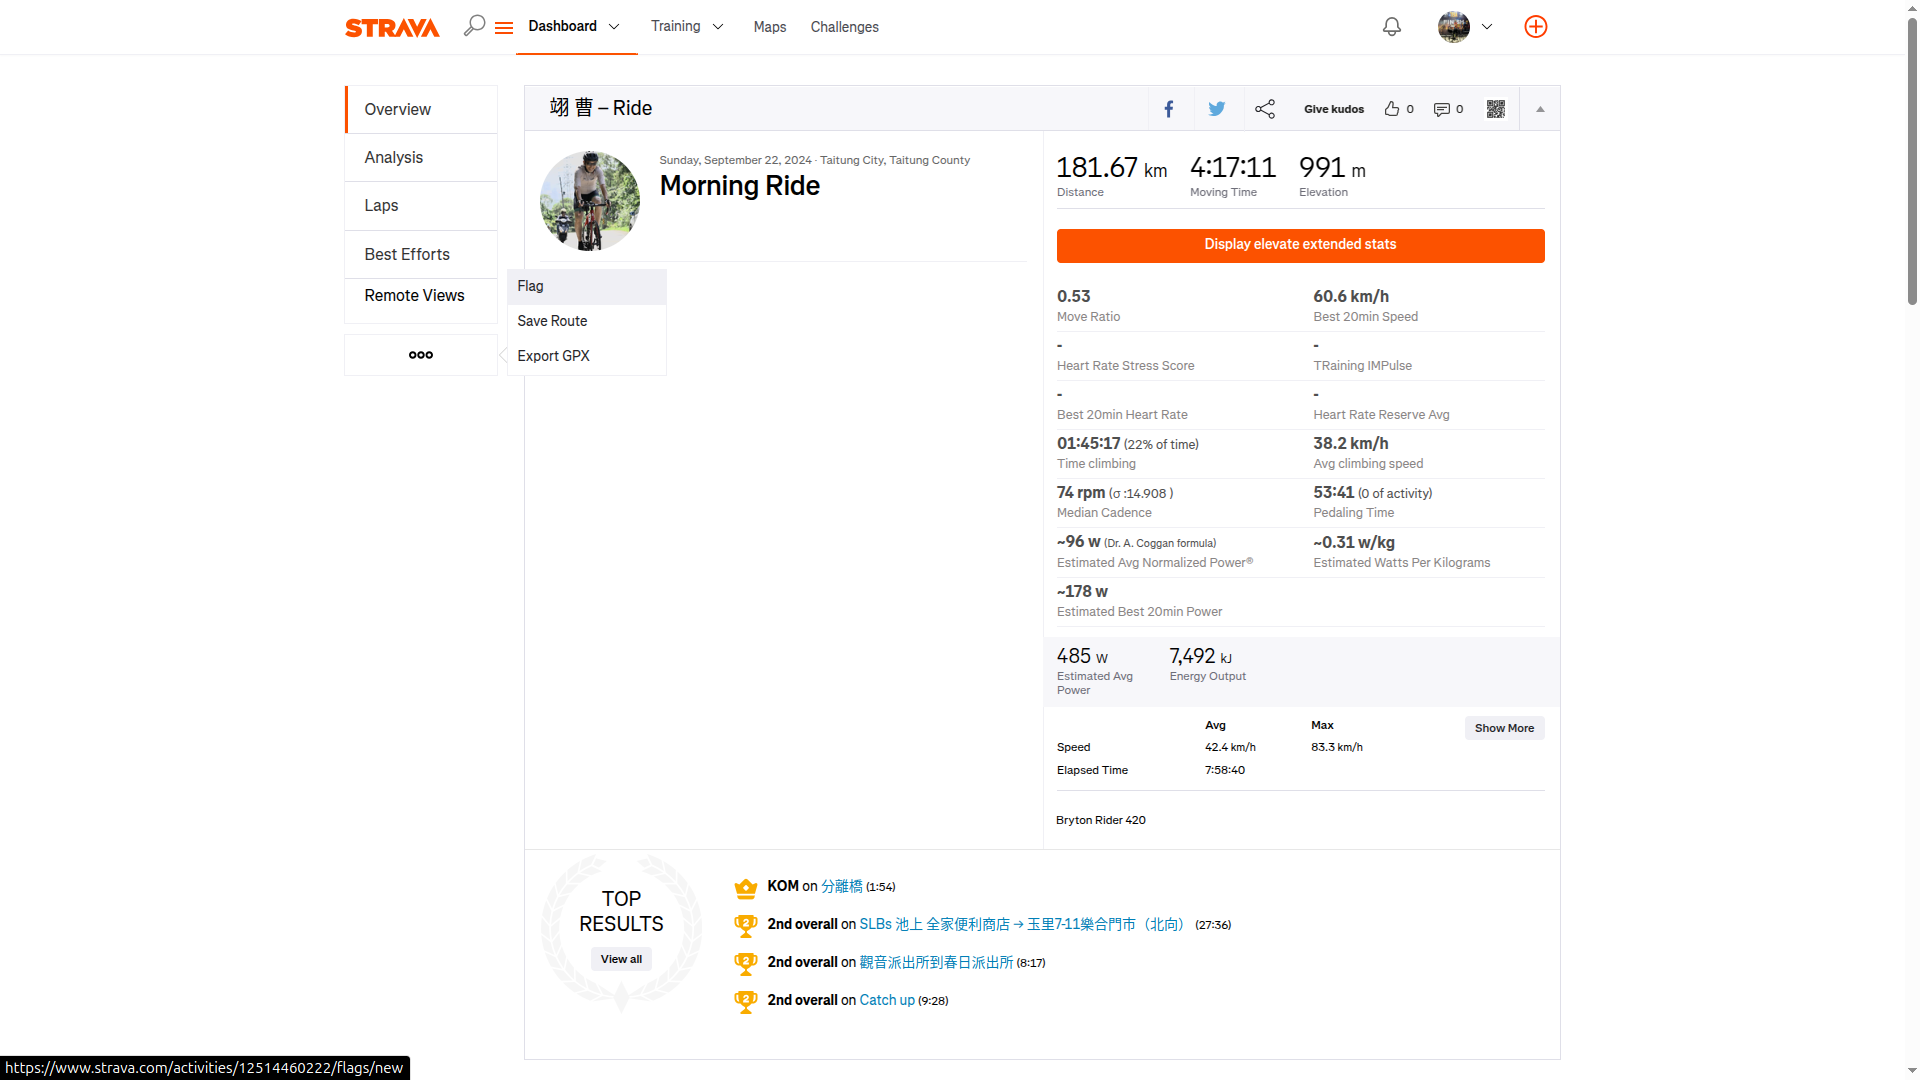
\includegraphics[width=7cm]{flag1.png}
\item 點選檢舉類型並輸入原因:\\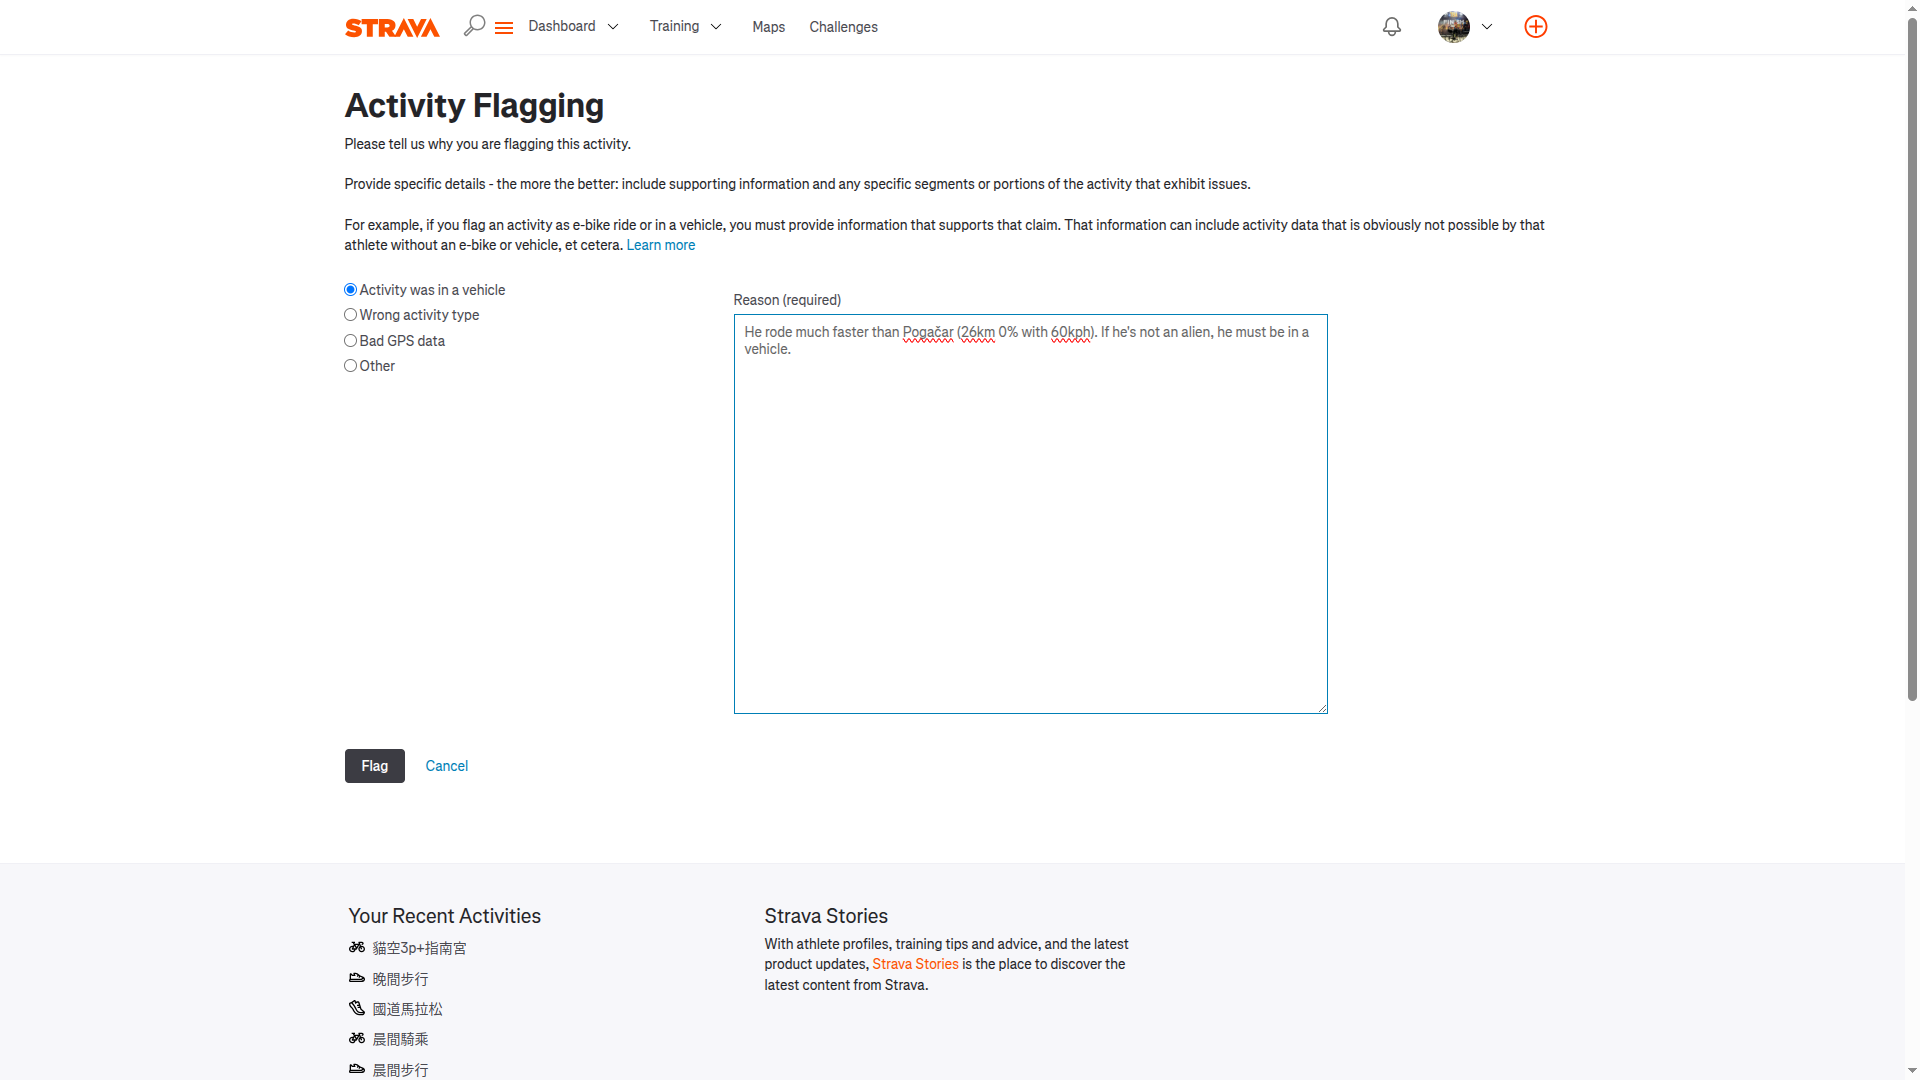
\includegraphics[width=7cm]{flag2.png}
}
\end{multicols}
\only<2>{
\item 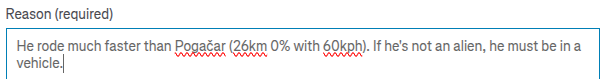
\includegraphics[width=14cm]{flag3.png}
}
\end{itemize}
\end{frame}

\begin{frame}{不要亂檢舉}
\begin{multicols}{2}
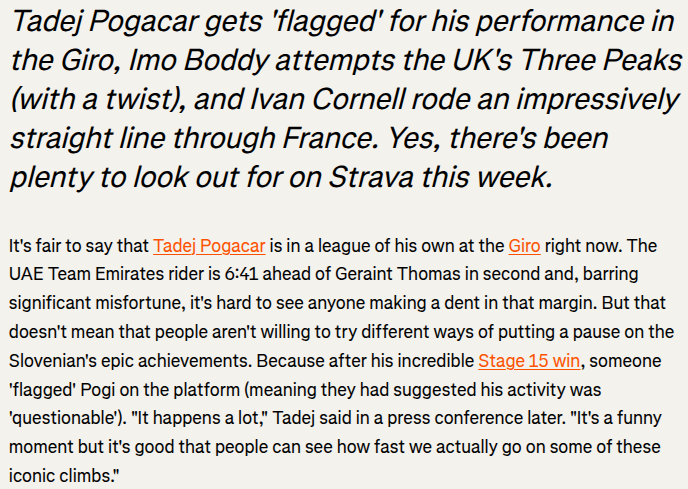
\includegraphics[width=7cm]{flag5.png}
\newpage

\includegraphics[width=7cm]{flag4.png}
\end{multicols}
\end{frame}
